\section{Lineare Algebra und Geometrie}
\subsection{Vektorrechnung}
\subsubsection{Vektoren in $\mathbb{R}^2 $ und $\mathbb{R}^3 $}

\begin{frame}{Skalare und Vektoren}
	\begin{definition}[Skalar]
		Eine Größe, die durch die Angabe einer einzigen (reellen) Zahl (mit evtl. einer Einheit) angegeben werden kann, heißt \textbf{Skalar}.
	\end{definition}
	Skalare sind zum Beispiel:
	\begin{itemize}
		\item Druck (z.B. 3,2 bar)
		\item Temperatur (z.B. $24^\circ$ Celsius)
		\item Dichte (z.B. $1000 \frac{g}{cm^3}$)
	\end{itemize}
	\begin{definition}[Vektor]
		Eine Größe, die nur durch die Angabe einer (reellen) Zahl (mit evtl. einer Einheit) \textbf{und einer Richtung} angegeben werden kann, heißt \textbf{Vektor}.
	\end{definition}
	Vektoren sind zum Beispiel:
	\begin{itemize}
		\item Kraft (Gewichtskraft $100$ N in Richtung Erdmittelpunkt)
		\item Geschwindigkeit ($200 \frac{km}{h}$ in Richtung Norden)
		\item Drehmoment ($200$ Nm im Uhrzeigersinn)
	\end{itemize}	
\end{frame}

\begin{frame}{Darstellung von Vektoren}
	\begin{bemerkung}[zur Schreibweise]
		Vektoren werden (in der Regel) durch Angabe eines Vektorpfeiles gekennzeichnet:
		\begin{itemize}
			\item $\vv{a}$
			\item $\vv{OP}$ für den Vektor, der vom Punkt $O$ zum Punkt $P$ zeigt.
		\end{itemize}
	\end{bemerkung}
\definecolor{xdxdff}{rgb}{0.49019607843137253,0.49019607843137253,1.}
\definecolor{qqqqff}{rgb}{0.,0.,1.}
\definecolor{uuuuuu}{rgb}{0.26666666666666666,0.26666666666666666,0.26666666666666666}
\begin{tikzpicture}[line cap=round,line join=round,>=triangle 45,x=0.9cm,y=1.0cm]
\draw[->,color=black] (-2.6755555555555546,0.) -- (8.328888888888887,0.);
\foreach \x in {-2.5,-2.,-1.5,-1.,-0.5,0.5,1.,1.5,2.,2.5,3.,3.5,4.,4.5,5.,5.5,6.,6.5,7.,7.5,8.}
\draw[shift={(\x,0)},color=black] (0pt,2pt) -- (0pt,-2pt) node[below] {\footnotesize $\x$};
\draw[->,color=black] (0.,-1.9066666666666725) -- (0.,4.315555555555556);
\foreach \y in {-1.5,-1.,-0.5,0.5,1.,1.5,2.,2.5,3.,3.5,4.}
\draw[shift={(0,\y)},color=black] (2pt,0pt) -- (-2pt,0pt) node[left] {\footnotesize $\y$};
\draw[color=black] (0pt,-10pt) node[right] {\footnotesize $0$};
\clip(-2.6755555555555546,-1.9066666666666725) rectangle (8.328888888888887,4.315555555555556);
\draw [->,line width=1.2pt] (0.,0.) -- (2.,3.);
\draw [->,line width=1.2pt] (2.,0.) -- (4.,3.);
\begin{scriptsize}
\draw [fill=uuuuuu] (0.,0.) circle (1.5pt);
\draw[color=qqqqff] (0.26222222222222272,0.12888888888888497) node {$O$};
\draw [fill=qqqqff] (2.,3.) circle (1.5pt);
\draw[color=qqqqff] (2.2622222222222226,3.1244444444444435) node {$A$};
\draw [fill=xdxdff] (2.,0.) circle (1.5pt);
\draw[color=qqqqff] (2.2622222222222226,0.12888888888888497) node {$B$};
\draw [fill=qqqqff] (4.,3.) circle (1.5pt);
\draw[color=qqqqff] (4.262222222222221,3.1244444444444435) node {$C$};
\draw[color=black] (1.4222222222222226,1.595555555555553) node {$\vv{OA}$};
\draw[color=black] (3.422222222222222,1.595555555555553) node {$\vv{BC}$};
\end{scriptsize}
\end{tikzpicture}
\end{frame}

\begin{frame}{Koordinaten eines Vektors}
	Da ein Vektor eine Richtung hat, braucht man ein Koordinatensystem und gibt den Vektor in Koordinaten wie folgt an:
	
	\definecolor{xdxdff}{rgb}{0.49019607843137253,0.49019607843137253,1.}
	\definecolor{qqqqff}{rgb}{0.,0.,1.}
	\definecolor{uuuuuu}{rgb}{0.26666666666666666,0.26666666666666666,0.26666666666666666}
	\begin{tikzpicture}[line cap=round,line join=round,>=triangle 45,x=0.9cm,y=1.0cm]
	\draw[->,color=black] (-2.6755555555555546,0.) -- (8.328888888888887,0.);
	\foreach \x in {-2.5,-2.,-1.5,-1.,-0.5,0.5,1.,1.5,2.,2.5,3.,3.5,4.,4.5,5.,5.5,6.,6.5,7.,7.5,8.}
	\draw[shift={(\x,0)},color=black] (0pt,2pt) -- (0pt,-2pt) node[below] {\footnotesize $\x$};
	\draw[->,color=black] (0.,-1.9066666666666725) -- (0.,4.315555555555556);
	\foreach \y in {-1.5,-1.,-0.5,0.5,1.,1.5,2.,2.5,3.,3.5,4.}
	\draw[shift={(0,\y)},color=black] (2pt,0pt) -- (-2pt,0pt) node[left] {\footnotesize $\y$};
	\draw[color=black] (0pt,-10pt) node[right] {\footnotesize $0$};
	\clip(-2.6755555555555546,-1.9066666666666725) rectangle (8.328888888888887,4.315555555555556);
	\draw [->,line width=1.2pt] (0.,0.) -- (2.,3.);
	\draw [line width=1.2pt,dash pattern=on 2pt off 2pt] (2.,3.)-- (2.,0.);
	\draw [line width=1.2pt,dash pattern=on 1pt off 1pt] (2.,3.)-- (0.,3.);
	\begin{scriptsize}
	\draw [fill=uuuuuu] (0.,0.) circle (1.5pt);
	\draw[color=uuuuuu] (0.06222222222222272,0.12888888888888497) node {$O$};
	\draw [fill=qqqqff] (2.,3.) circle (1.5pt);
	\draw[color=qqqqff] (2.0622222222222226,3.1244444444444435) node {$A$};
	\draw[color=black] (3.2222222222222226,2.595555555555553) node {$\vv{a}=\vv{OA}=\begin{pmatrix}2 \\ 3\end{pmatrix}$};
	\draw [fill=xdxdff] (2.,0.) circle (1.5pt);
	\draw[color=xdxdff] (2.0622222222222226,0.12888888888888497) node {$x_A$};
	\draw[color=black] (1.9022222222222225,1.6044444444444421) node {$p_x$};
	\draw [fill=xdxdff] (0.,3.) circle (1.5pt);
	\draw[color=xdxdff] (0.06222222222222272,3.1244444444444435) node {$y_A$};
	\draw[color=black] (1.04,3.2488888888888883) node {$p_y$};
	\end{scriptsize}
	\end{tikzpicture}
\end{frame}

\begin{frame}{Koordinaten eines Vektors}
	Und genauso dreidimensional:
	$\vv{OA}=\begin{pmatrix}
	3 \\ -4 \\ 3
	\end{pmatrix}$
	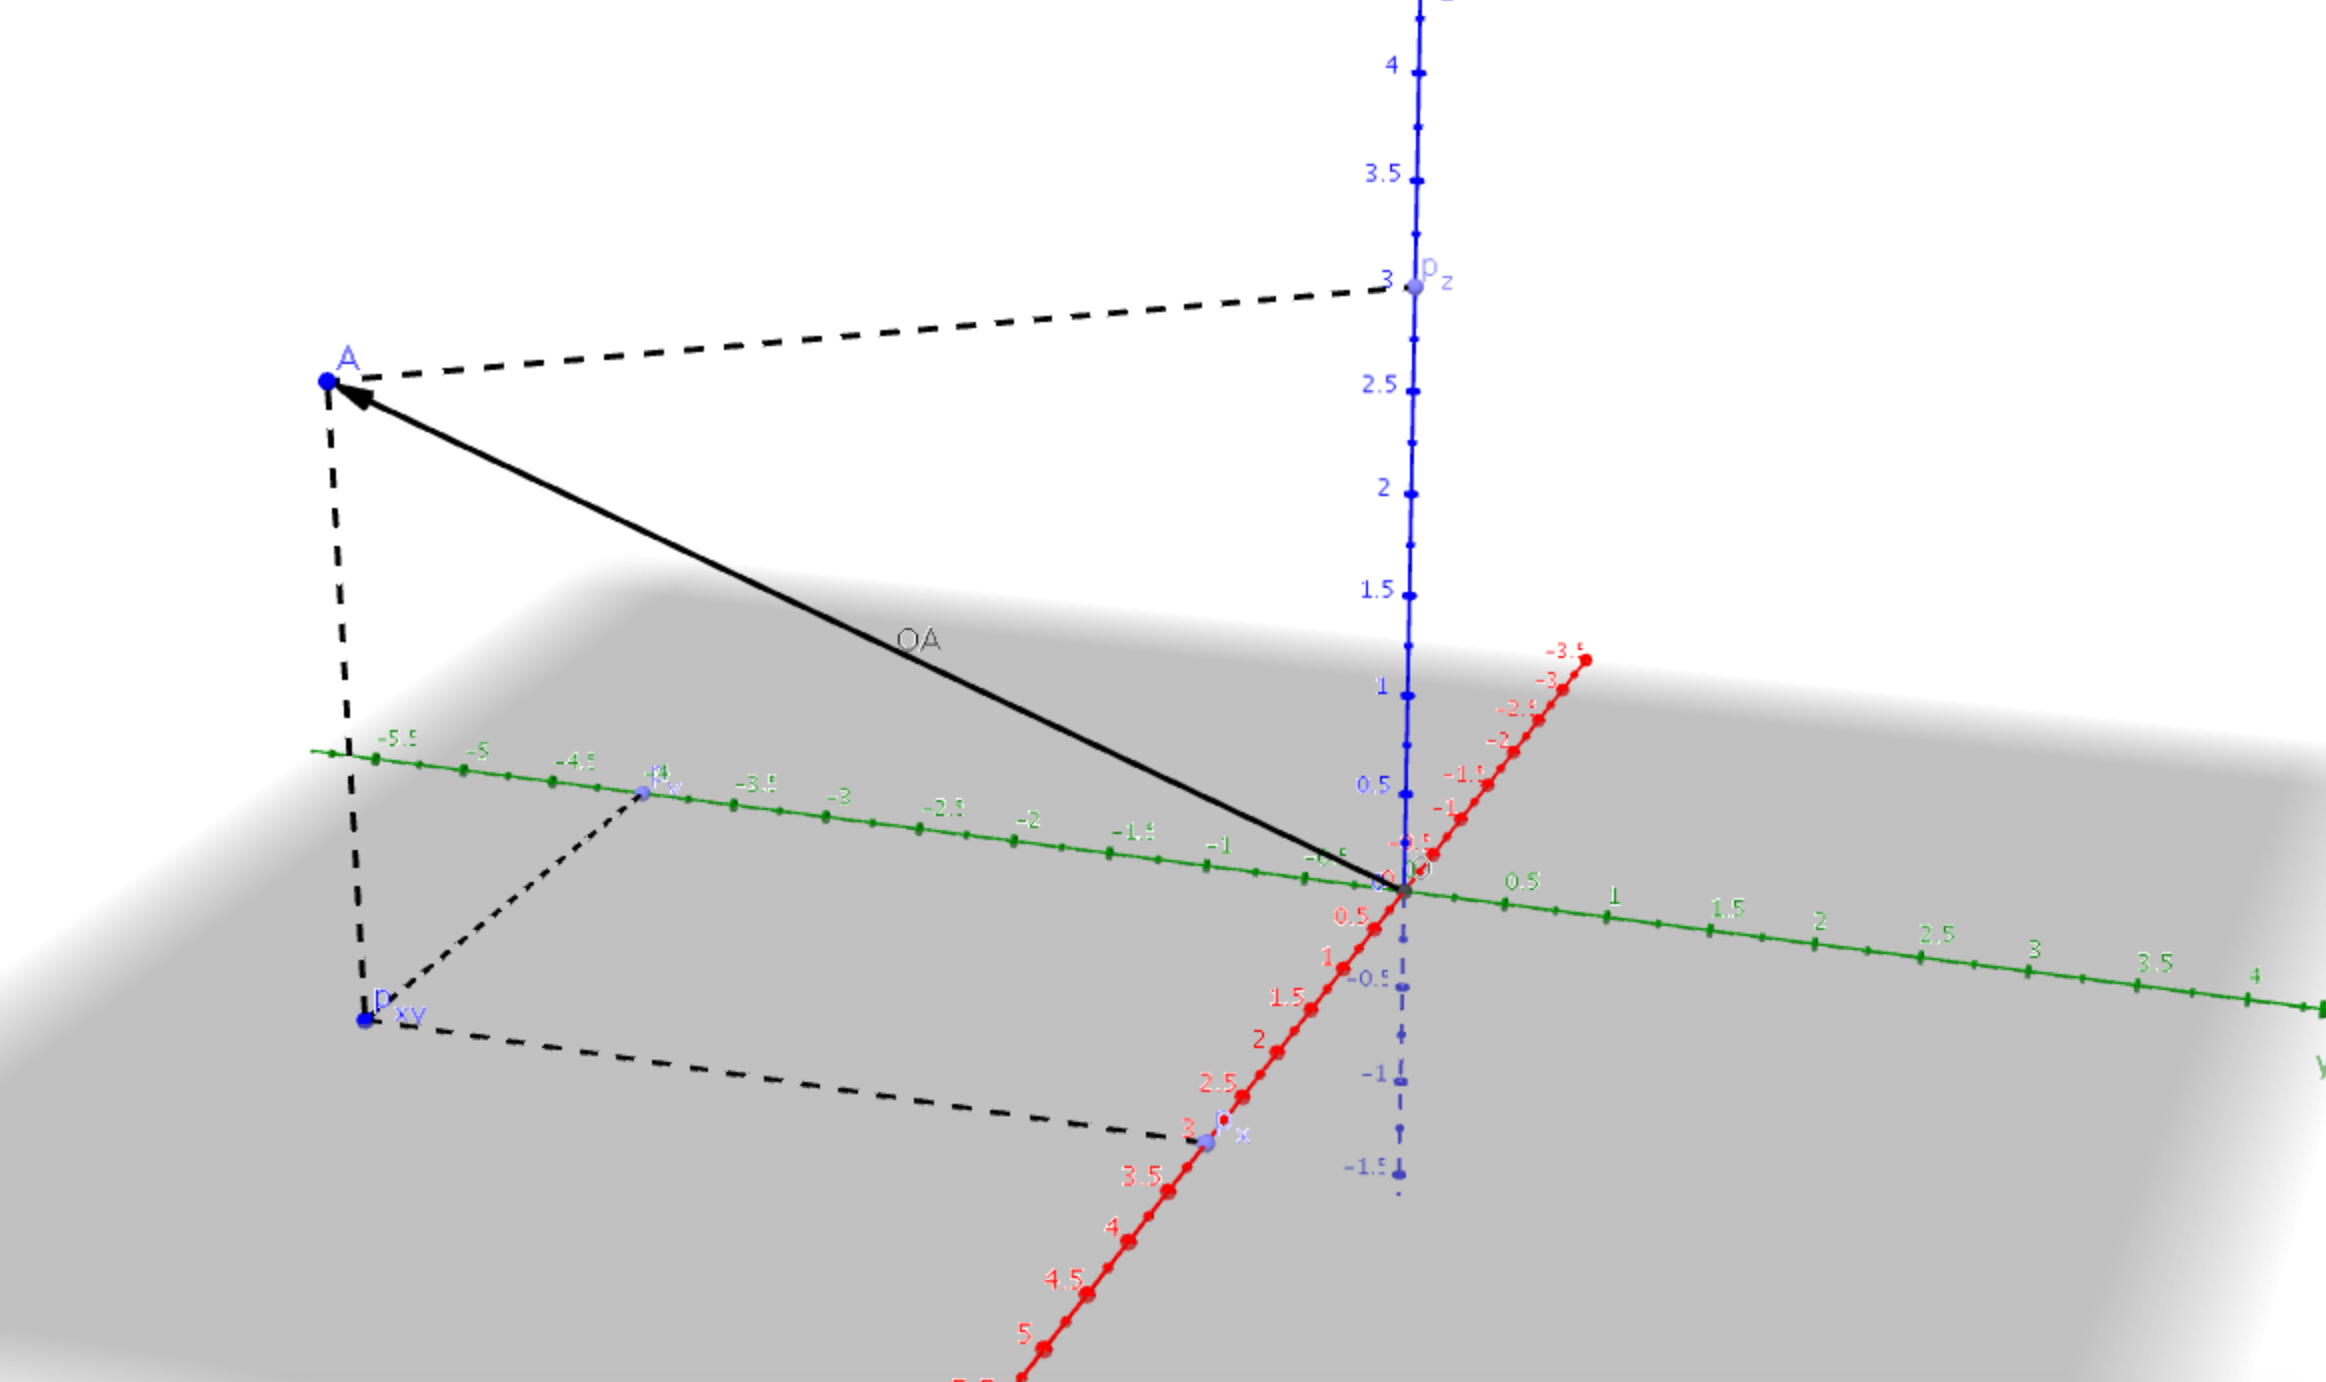
\includegraphics[width=10cm]{koordinaten3d.png}
\end{frame}

\begin{frame}{Schreibweise}
	\begin{bemerkung}[Koordinaten]
		Die Koordinaten von Vektoren werden wie folgt bezeichnet:
		\[
			\vv{a} = \begin{pmatrix}
			a_x \\ a_y \\ a_z
				\end{pmatrix} = \begin{pmatrix}
				a_1 \\ a_2 \\ a_3
				\end{pmatrix} \in \mathbb{R}^3
		\]
		für dreidimensionale Vektoren beziehungsweise
				\[
				\vv{b} = \begin{pmatrix}
				b_x \\ b_y
				\end{pmatrix} = \begin{pmatrix}
				b_1 \\ b_2
				\end{pmatrix} \in \mathbb{R}^2
				\]
		wenn der Vektor nur zweidimensional ist.
				
	\end{bemerkung}
\end{frame}

\begin{frame}{Schreibweise}
	\begin{bemerkung}[Koordinaten]
		Ganz allgemein werden die Koordinaten von Vektoren auch in höheren Dimensionen wie folgt bezeichnet:
		\[
		\vv{a} = \begin{pmatrix}
		a_1 \\ a_2 \\ \vdots \\ a_n
		\end{pmatrix} \in \mathbb{R}^{n}
		\]
		für n-dimensionale Vektoren.
	\end{bemerkung}
\end{frame}


\begin{frame}{Gleichheit von Vektoren}
	\begin{bemerkung}[Gleichheit von Vektoren]
		Zwei Vektoren sind schon dann \textbf{gleich}, wenn Sie dieselbe Länge (Betrag) und dieselbe Richtung haben!
	\end{bemerkung}
		\definecolor{xdxdff}{rgb}{0.49019607843137253,0.49019607843137253,1.}
		\definecolor{qqqqff}{rgb}{0.,0.,1.}
		\definecolor{uuuuuu}{rgb}{0.26666666666666666,0.26666666666666666,0.26666666666666666}
		\begin{tikzpicture}[line cap=round,line join=round,>=triangle 45,x=0.85cm,y=1.0cm]
		\draw[->,color=black] (-2.18,0.) -- (9.286666666666669,0.);
		\foreach \x in {-2.,-1.,1.,2.,3.,4.,5.,6.,7.,8.,9.}
		\draw[shift={(\x,0)},color=black] (0pt,2pt) -- (0pt,-2pt) node[below] {\footnotesize $\x$};
		\draw[->,color=black] (0.,-3.6866666666666705) -- (0.,4.94);
		\foreach \y in {-3.,-2.,-1.,1.,2.,3.,4.}
		\draw[shift={(0,\y)},color=black] (2pt,0pt) -- (-2pt,0pt) node[left] {\footnotesize $\y$};
		\draw[color=black] (0pt,-10pt) node[right] {\footnotesize $0$};
		\clip(-2.18,-3.6866666666666705) rectangle (9.286666666666669,4.94);
		\draw [ultra thick, ->] (0.,0.) -- (2.,4.);
		\draw [ultra thick, ->] (2.,0.) -- (4.,4.);
		\begin{scriptsize}
		\draw [fill=uuuuuu] (0.,0.) circle (1.5pt);
		\draw[color=qqqqff] (0.3,0.19333333333333036) node {$O$};
		\draw [fill=qqqqff] (2.,4.) circle (1.5pt);
		\draw[color=qqqqff] (2.3,4.193333333333331) node {$A$};
		\draw [fill=xdxdff] (2.,0.) circle (1.5pt);
		\draw[color=qqqqff] (2.3,0.19333333333333036) node {$B$};
		\draw [fill=qqqqff] (4.,4.) circle (1.5pt);
		\draw[color=qqqqff] (4.3,4.193333333333331) node {$C$};
		\draw[color=black] (2.1,2.14) node {\large $\vv{u}=\begin{pmatrix} 2 \\ 4 \end{pmatrix}$};
		\draw[color=black] (4.8,2.14) node {\large $\vv{v}=\begin{pmatrix} 2 \\ 4 \end{pmatrix} = \vv{u}$};
		\end{scriptsize}
		\end{tikzpicture}
\end{frame}


\begin{frame}{Ortsvektoren}
	Einen Vektor, der vom Ursprung des Koordinatensystems $O$ zu einem Punkt $P=\begin{pmatrix}p_1 \\ p_2 \\ \vdots \\ p_n \end{pmatrix}$ gerichtet ist, bezeichnet man als \textbf{Ortsvektor des Punktes $P$} und schreibt:
	\[
		\vv{OP} = \begin{pmatrix}
		p_1 \\ p_2 \\ \vdots \\ p_n
		\end{pmatrix}
	\]
	Die Bezeichnung $\begin{pmatrix}
	p_1 \\ p_2 \\ \vdots \\ p_n
	\end{pmatrix}$
	steht also sowohl für den Punkt $P$ als auch für den Ortsvektor dieses Punktes.
\end{frame}


\begin{frame}{Summe und Differenz von Vektoren}
	Vektoren werden koordinatenweise addiert bzw. subtrahiert:
	\[
	\vv{a} + \vv{b} = \begin{pmatrix} a_x \\ a_y \\ a_z
	\end{pmatrix} + \begin{pmatrix} b_x \\ b_y \\ b_z
	\end{pmatrix} = \begin{pmatrix} a_x + b_x \\ a_y + b_y \\ a_z + b_z
	\end{pmatrix}
	\]
		\[
		\vv{a} - \vv{b} = \begin{pmatrix} a_x \\ a_y \\ a_z
		\end{pmatrix} - \begin{pmatrix} b_x \\ b_y \\ b_z
		\end{pmatrix} = \begin{pmatrix} a_x - b_x \\ a_y - b_y \\ a_z - b_z
		\end{pmatrix}
		\]
	und entsprechend für n-dimensionale Vektoren.	
\end{frame}

\begin{frame}{Summe und Differenz von Vektoren}
	
	\begin{displaymath}
		\vv{a} = \vv{u} - \vv{v} = \begin{pmatrix}
		2 \\ 1
		\end{pmatrix} - \begin{pmatrix}
		2 \\ 3
		\end{pmatrix} = \begin{pmatrix} 0 \\ -2
		\end{pmatrix}
		\end{displaymath}
		\begin{displaymath}
		\vv{w} = \vv{u} + \vv{v} = \begin{pmatrix}
		2 \\ 1
		\end{pmatrix} + \begin{pmatrix}
		2 \\ 3
		\end{pmatrix} = \begin{pmatrix} 4 \\ 4
		\end{pmatrix}
	\end{displaymath}
\definecolor{qqqqff}{rgb}{0.,0.,1.}
\definecolor{uuuuuu}{rgb}{0.26666666666666666,0.26666666666666666,0.26666666666666666}
\begin{tikzpicture}[line cap=round,line join=round,>=triangle 45,x=0.9cm,y=1.0cm]
\draw[->,color=black] (-1.3577777777777764,0.) -- (9.486666666666665,0.);
\foreach \x in {-1.,-0.5,0.5,1.,1.5,2.,2.5,3.,3.5,4.,4.5,5.,5.5,6.,6.5,7.,7.5,8.,8.5,9.}
\draw[shift={(\x,0)},color=black] (0pt,2pt) -- (0pt,-2pt) node[below] {\footnotesize $\x$};
\draw[->,color=black] (0.,-1.262222222222225) -- (0.,4.995555555555551);
\foreach \y in {-1.,-0.5,0.5,1.,1.5,2.,2.5,3.,3.5,4.,4.5}
\draw[shift={(0,\y)},color=black] (2pt,0pt) -- (-2pt,0pt) node[left] {\footnotesize $\y$};
\draw[color=black] (0pt,-10pt) node[right] {\footnotesize $0$};
\clip(-1.3577777777777764,-1.262222222222225) rectangle (9.486666666666665,4.995555555555551);
\draw [ultra thick, ->] (0.,0.) -- (2.,1.);
\draw [ultra thick, ->] (0.,0.) -- (2.,3.);
\draw [ultra thick, ->] (2.,1.) -- (4.,4.);
\draw [ultra thick, ->] (2.,3.) -- (2.,1.);
\begin{scriptsize}
\draw [fill=uuuuuu] (0.,0.) circle (1.5pt);
\draw[color=uuuuuu] (0.06444444444444544,0.12444444444444139) node {$A$};
\draw [fill=qqqqff] (2.,1.) circle (1.5pt);
\draw[color=qqqqff] (2.064444444444445,1.1288888888888857) node {$B$};
\draw[color=black] (1.1066666666666675,0.8044444444444413) node {$\vv{u}$};
\draw[ultra thick, ->] (0., 0.) -- (4.,4.);
\draw[color=black] (2.5, 2.7) node {$\vv{w}$};
\draw [fill=qqqqff] (2.,3.) circle (1.5pt);
\draw[color=qqqqff] (2.064444444444445,3.128888888888885) node {$C$};
\draw[color=black] (1.1977777777777785,1.5911111111111078) node {$\vv{v}$};
\draw [fill=qqqqff] (4.,4.) circle (1.5pt);
\draw[color=qqqqff] (4.064444444444445,4.12444444444444) node {$D$};
\draw[color=black] (3.1977777777777783,2.595555555555552) node {$\vv{v}$};
\draw[color=black] (1.7555555555555562,2.08) node {$\vv{a}$};
\end{scriptsize}
\end{tikzpicture}
%\begin{tikzpicture}
%\begin{axis}[title=Differenz zweier Vektoren]
%\addplot[blue,
%quiver={u=\thisrow{u},v=\thisrow{v}},-stealth,ultra thick]
%table[row sep=\\]
%{
%x y u v
%0 0 1 0\\
%0 0 1 0\\
%0 0 0 1\\
%0 1 1 -1\\
%};
%\end{axis}
%\end{tikzpicture}
\end{frame}

\begin{frame}{Vektoren 3-dimensional}
	Dasselbe gilt natürlich auch für dreidimensionale Vektoren!
	\[
	\vv{u} + \vv{v} = \begin{pmatrix}
	0 \\ 1 \\ 2
	\end{pmatrix} + \begin{pmatrix}
	2 \\ 1 \\ 0
	\end{pmatrix} = \begin{pmatrix}
	2 \\ 2 \\ 2
	\end{pmatrix}
	\]
	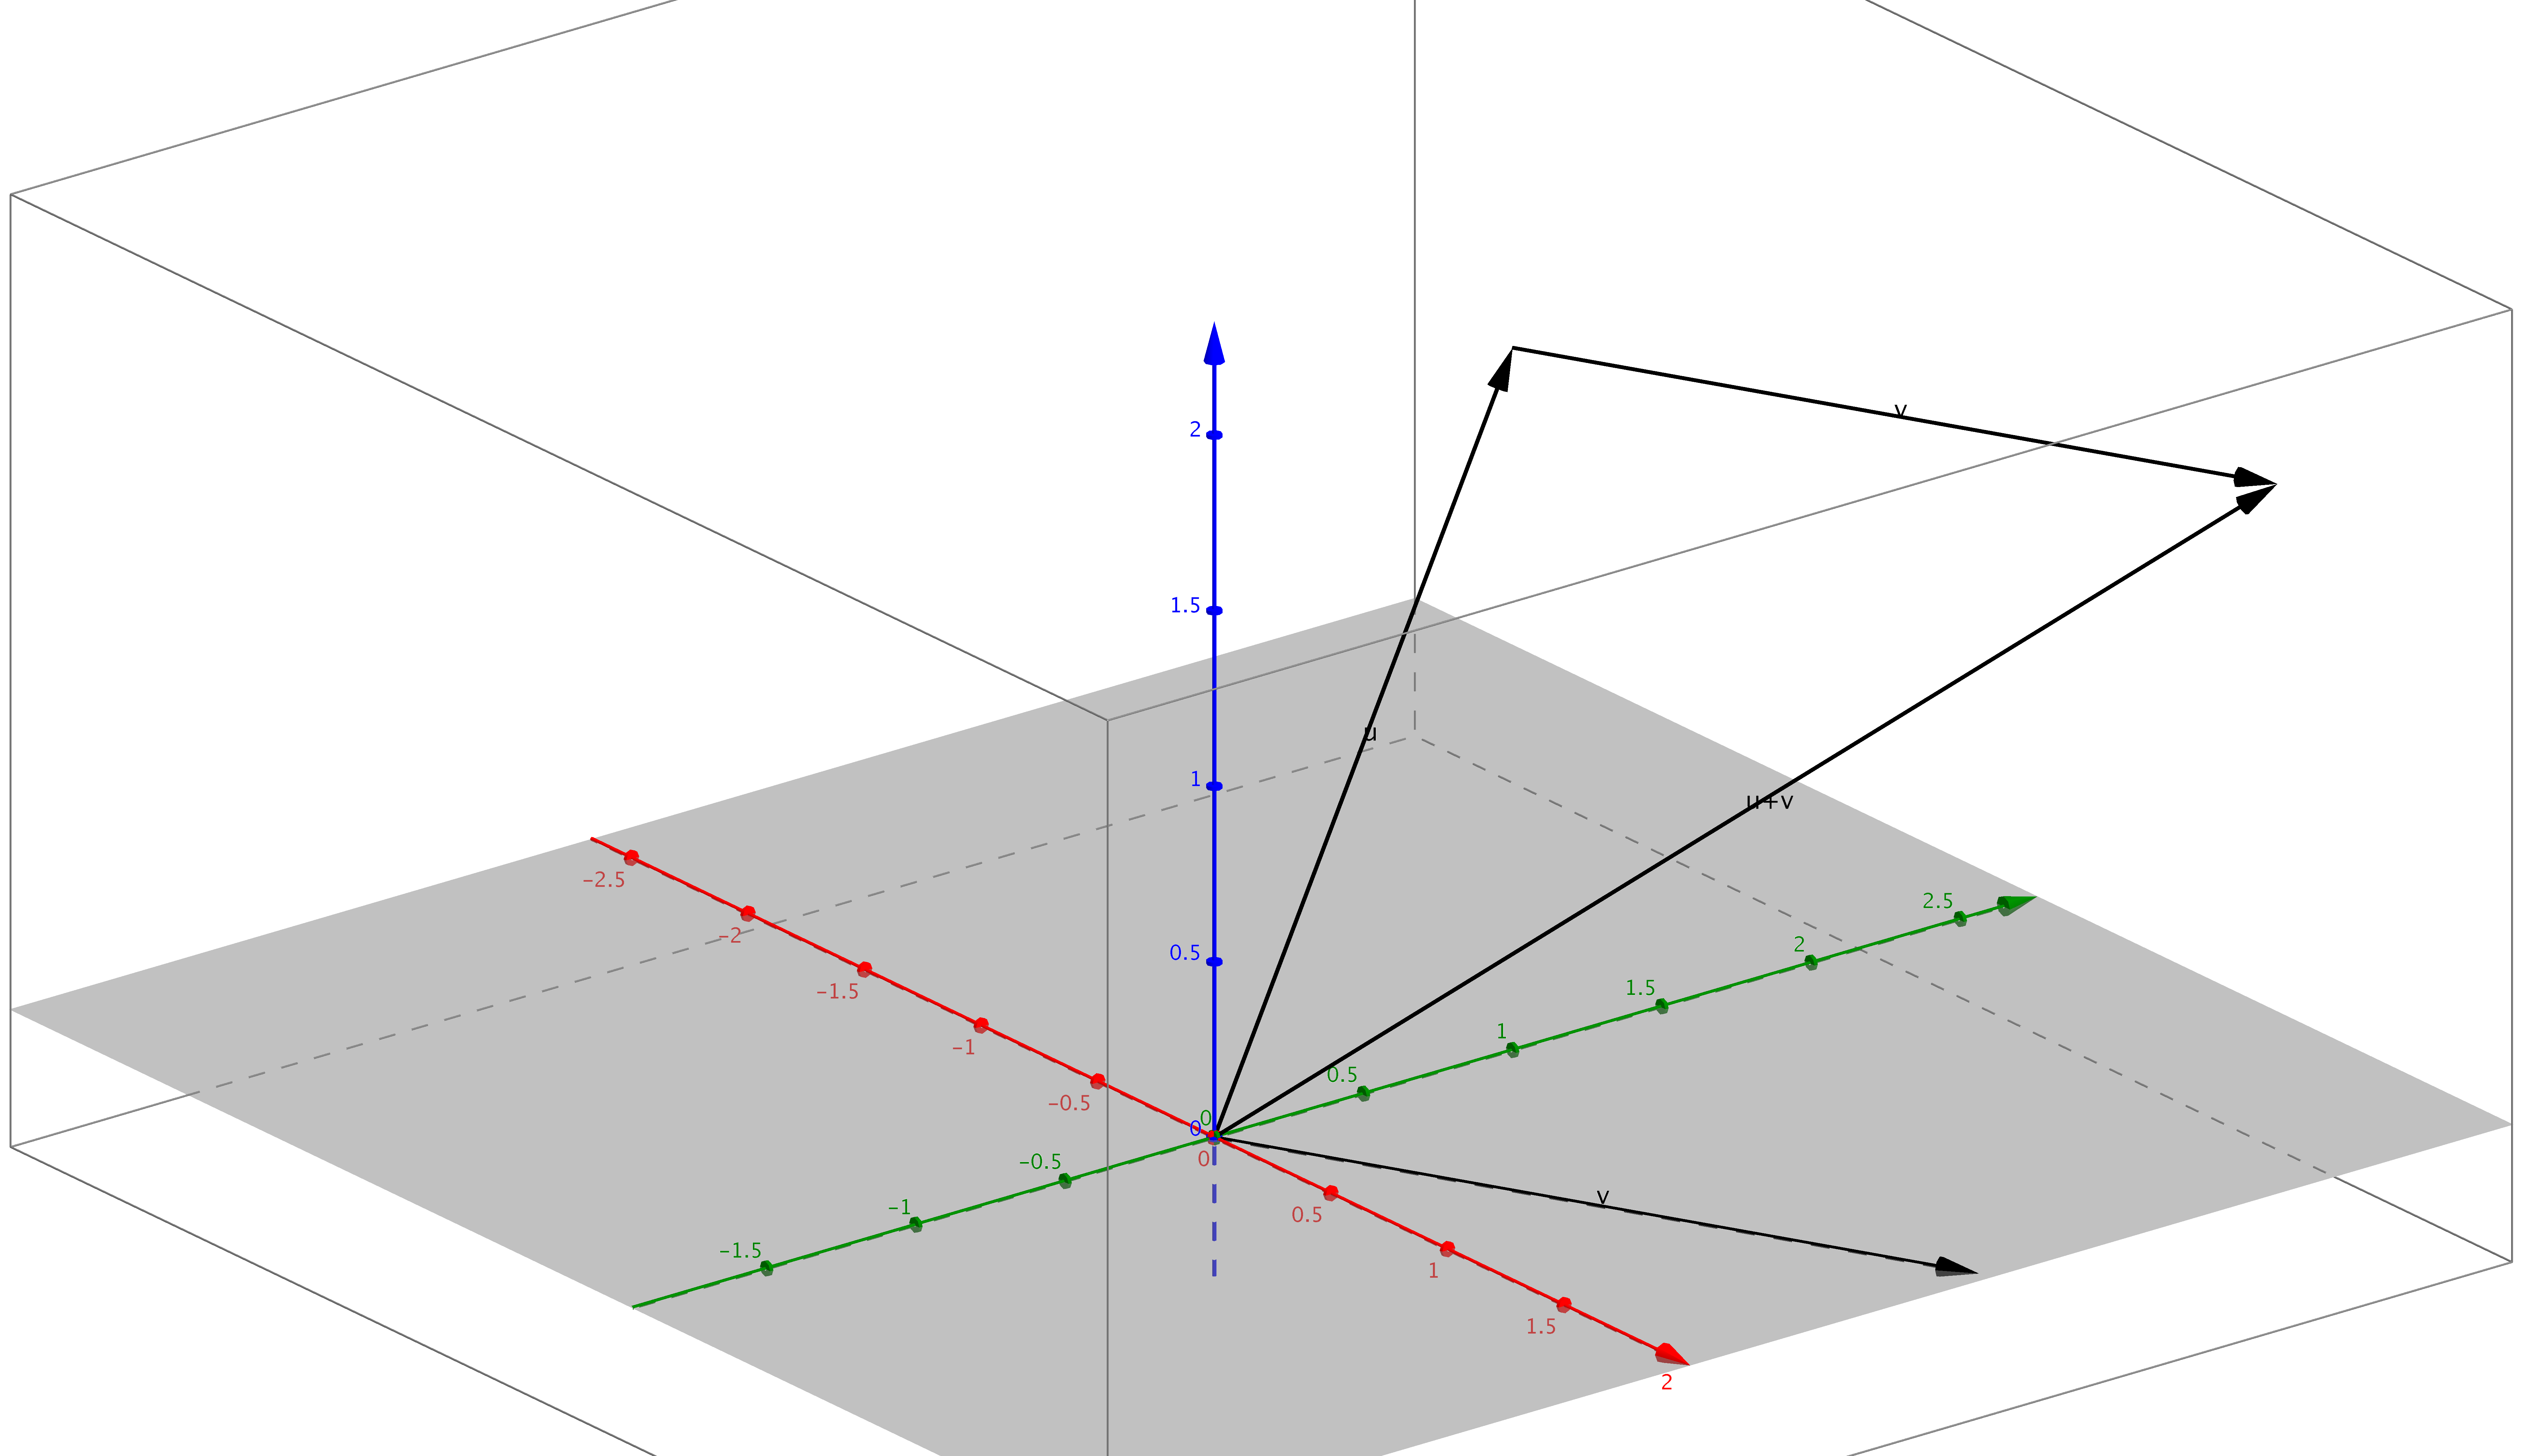
\includegraphics[width=10cm]{vektoren3d.png}
\end{frame}

\begin{frame}{Verlängern, Verkürzen und Umdrehen von Vektoren}
	Vektoren können mit Zahlen (Skalaren) multipliziert werden. Für eine Zahl $\lambda \in \mathbb{R}$ ist
	\[
		\lambda \vv{a} = \lambda \begin{pmatrix}a_x \\ a_y \\ a_z\end{pmatrix} = \begin{pmatrix}\lambda a_x \\ \lambda  a_y \\ \lambda a_z\end{pmatrix}
	\]
	und wieder entsprechend für n-dimensionale Vektoren.
\end{frame}

\begin{frame}{Multiplikation eines Vektors mit einem Skalar}
	Dabei gilt
	\begin{itemize}
	\item für $ | \lambda | > 1$ wird der Vektor verlängert/gestreckt.
	\item für $| \lambda |< 1$ wird der Vektor verkürzt/gestaucht.
	\item für $\lambda < 0$ wird die Richtung des Vektors zudem umgekehrt.
	\end{itemize}
	\definecolor{ffqqqq}{rgb}{1.,0.,0.}
	\definecolor{qqqqff}{rgb}{0.,0.,1.}
	\definecolor{uuuuuu}{rgb}{0.26666666666666666,0.26666666666666666,0.26666666666666666}
	\definecolor{cqcqcq}{rgb}{0.7529411764705882,0.7529411764705882,0.7529411764705882}
	\begin{tikzpicture}[line cap=round,line join=round,>=triangle 45,x=1.0cm,y=1.0cm]
	\draw [color=cqcqcq,, xstep=1.0cm,ystep=1.0cm] (-2.,-2.072292859071836) grid (7.,3.147259750704469);
	\draw[->,color=black] (-2.,0.) -- (7.,0.);
	\foreach \x in {-2.,-1.,1.,2.,3.,4.,5.,6.}
	\draw[shift={(\x,0)},color=black] (0pt,2pt) -- (0pt,-2pt) node[below] {\footnotesize $\x$};
	\draw[->,color=black] (0.,-2.072292859071836) -- (0.,3.147259750704469);
	\foreach \y in {-2.,-1.,1.,2.,3.}
	\draw[shift={(0,\y)},color=black] (2pt,0pt) -- (-2pt,0pt) node[left] {\footnotesize $\y$};
	\draw[color=black] (0pt,-10pt) node[right] {\footnotesize $0$};
	\clip(-2.,-2.072292859071836) rectangle (7.,3.147259750704469);
	\draw [->,line width=3.6pt] (0.,0.) -- (1.,2.);
	\draw [->,line width=1.2pt,color=ffqqqq] (0.,0.) -- (1.5,3.);
	\draw [->] (0.,0.) -- (-0.5,-1.);
	\begin{scriptsize}
	\draw [fill=uuuuuu] (0.,0.) circle (1.5pt);
	\draw[color=uuuuuu] (0.050538525269262585,0.1050062295777083) node {$O$};
	\draw [fill=qqqqff] (1.,2.) circle (1.5pt);
	\draw[color=qqqqff] (1.0497100248550122,2.1033492287492077) node {$A$};
	\draw[color=black] (1.1874067937033968,1.0892647217069542) node {$\vv{a}$};
	\draw [fill=qqqqff] (1.5,3.) circle (1.5pt);
	\draw[color=ffqqqq] (2.2900579950289974,2.3739374640433255) node {$\lambda \vv{a}$ für $\lambda = \frac{3}{2}$};
	\draw [fill=qqqqff] (-0.5,-1.) circle (1.5pt);
	\draw[color=qqqqff] (-0.4490472245236123,-0.8941652700080415) node {$C$};
	\draw[color=black] (1.0,-0.64677504631292964) node {$\lambda  \vv{a}$ für $\lambda = -\frac{1}{2}$ };
	\end{scriptsize}
	\end{tikzpicture}	
\end{frame}	

\subsubsection{Koordinaten}
\begin{frame}{Koordinatenvektoren}
	Die Vektoren der Länge 1 entlang der Koordinatenachsen haben eine spezielle Bezeichnung:
	\[
	\vv{e_x}=\begin{pmatrix} 1 \\ 0 \\ 0 \end{pmatrix} \quad 	\vv{e_y}=\begin{pmatrix} 0 \\ 1 \\ 0 \end{pmatrix} \quad
		\vv{e_z}=\begin{pmatrix} 0 \\ 0 \\ 1 \end{pmatrix}
	\]
	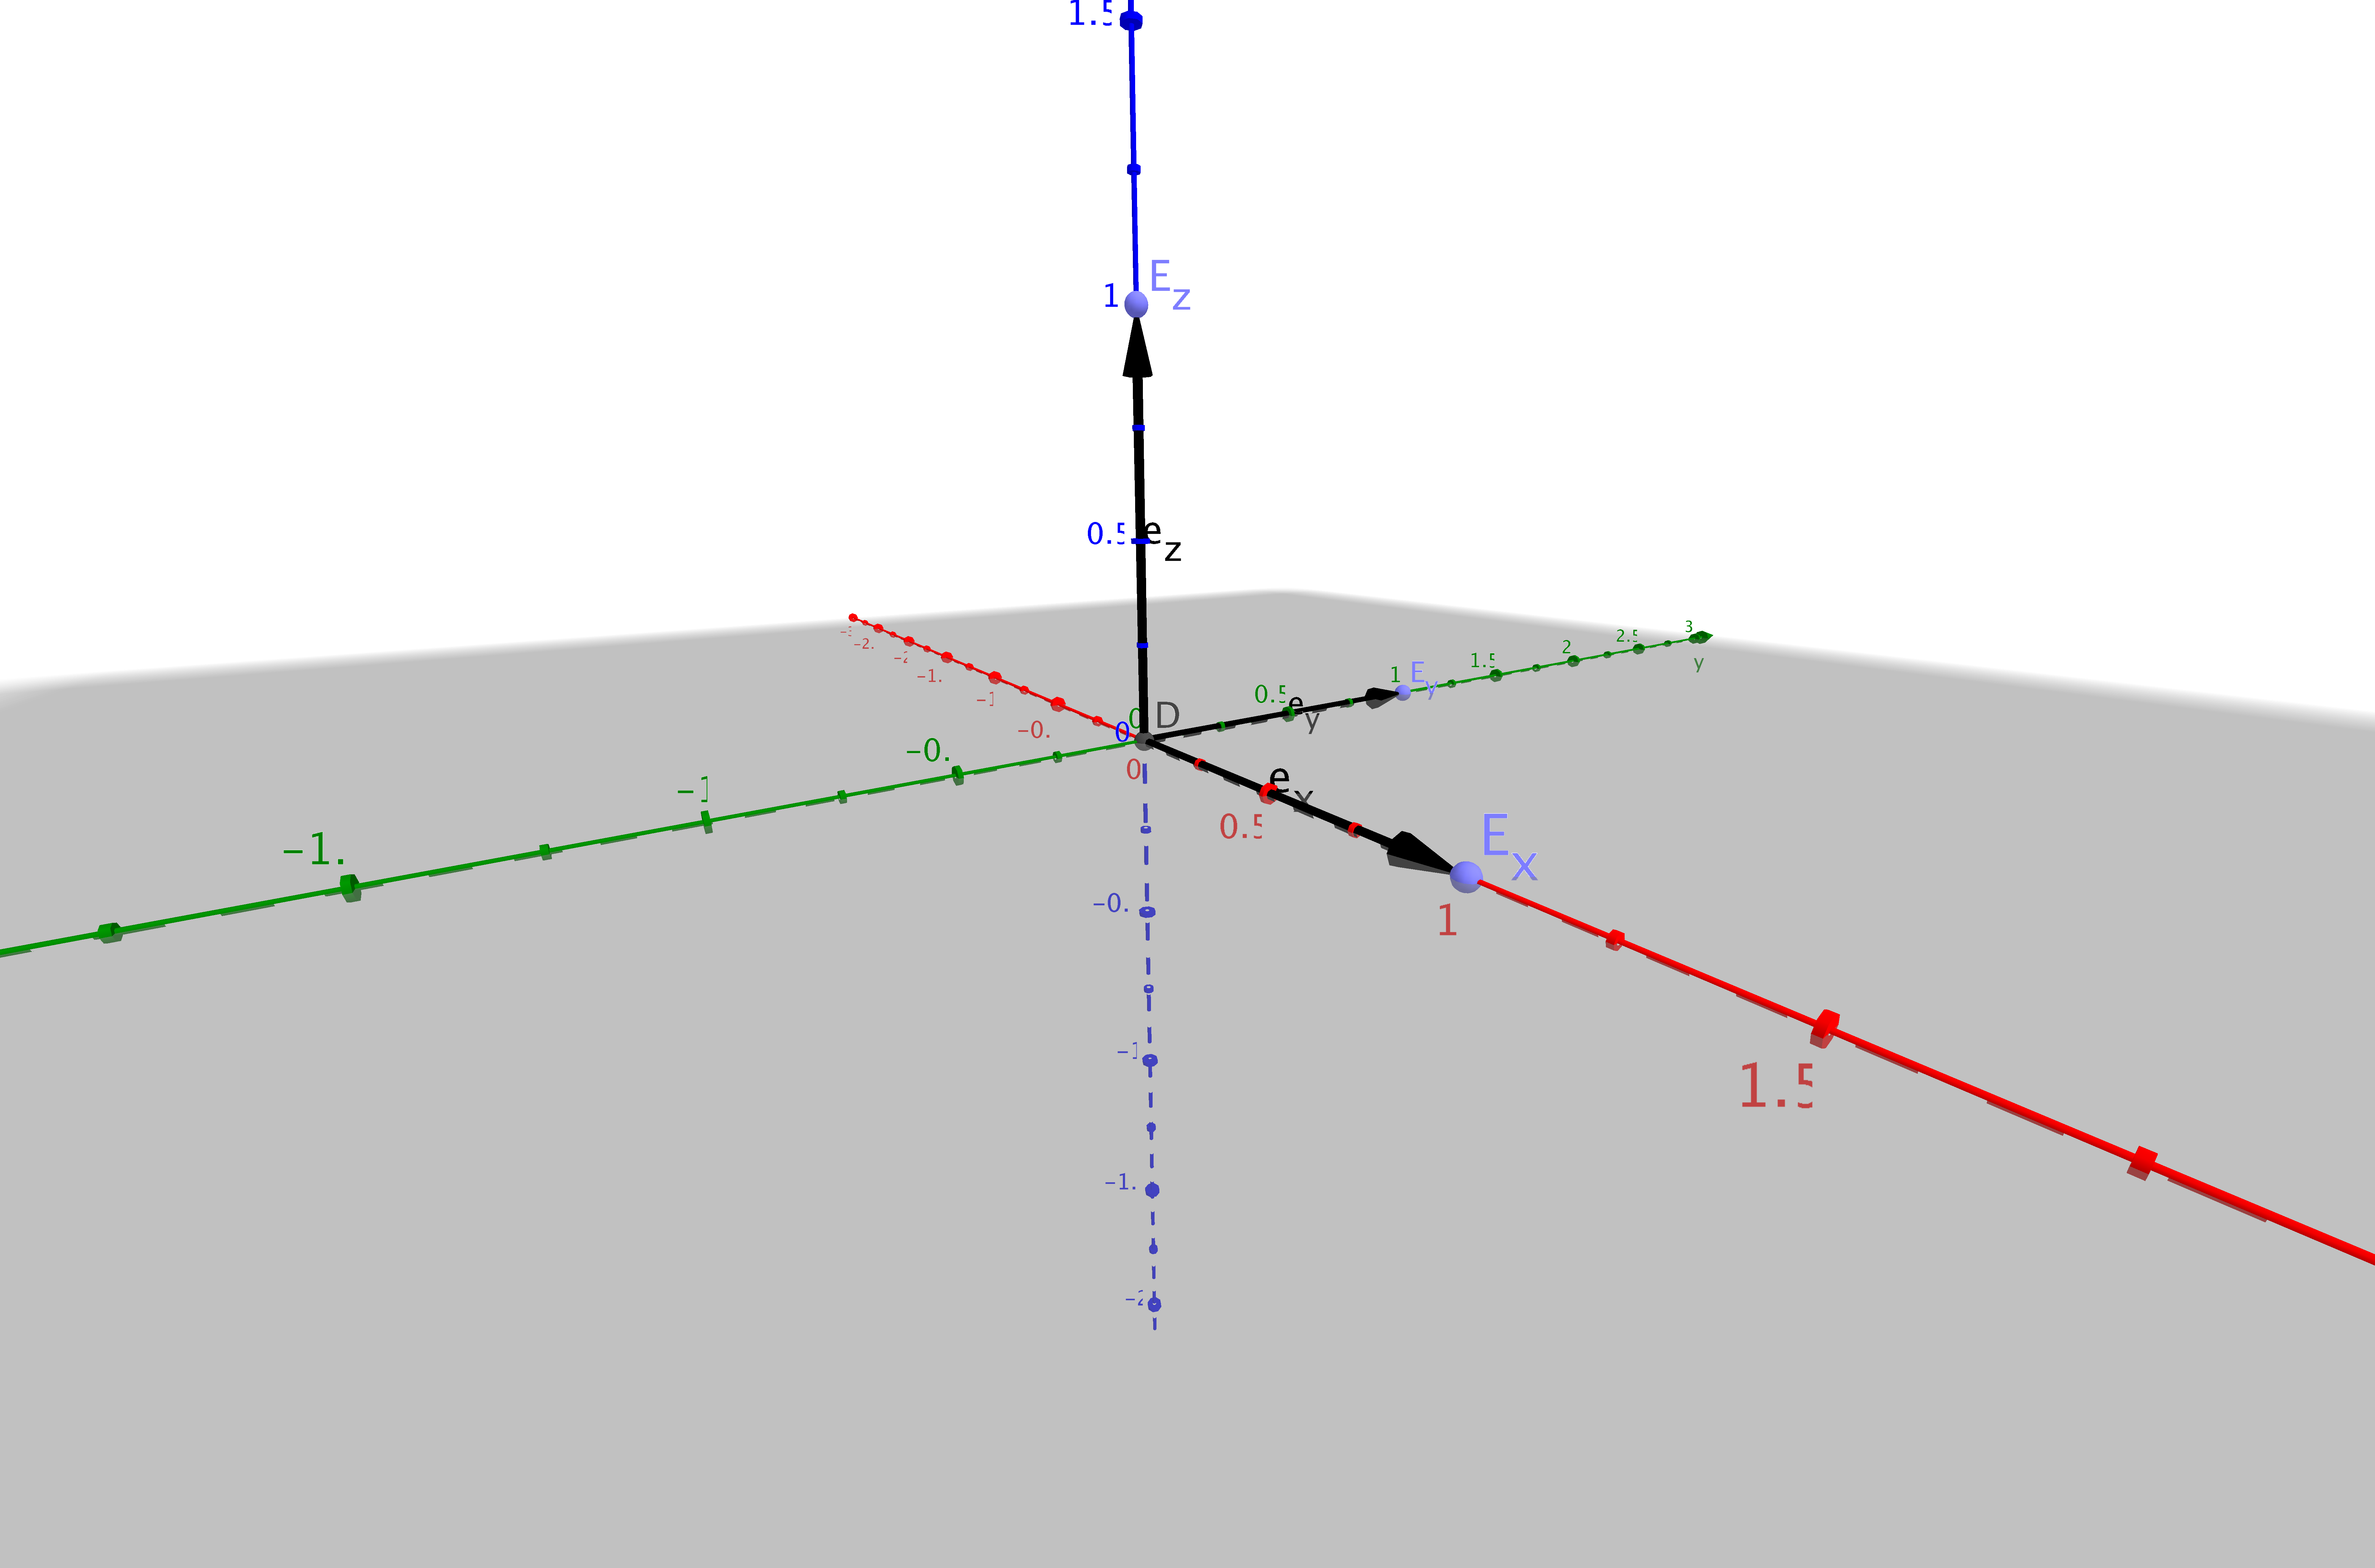
\includegraphics[width=10cm]{achsen.png}
\end{frame}

\begin{frame}{Projektionen}
	Mit Hilfe der Koordinatenvektoren kann man einen Vektor in seine Komponenten zerlegen:
	\[
	\begin{array}{cccc}
	\vv{OP} = \vv{a} = \begin{pmatrix}
	2 \\ 3 \\ 1
	\end{pmatrix} = &\underbrace{a_x \vv{e_x}} & + \underbrace{a_y \vv{e_y}}  + &\underbrace{a_z \vv{e_z}} \\
	&  \vv{a_x} & \vv{a_y} & \vv{a_z}
	\end{array}
	\]
	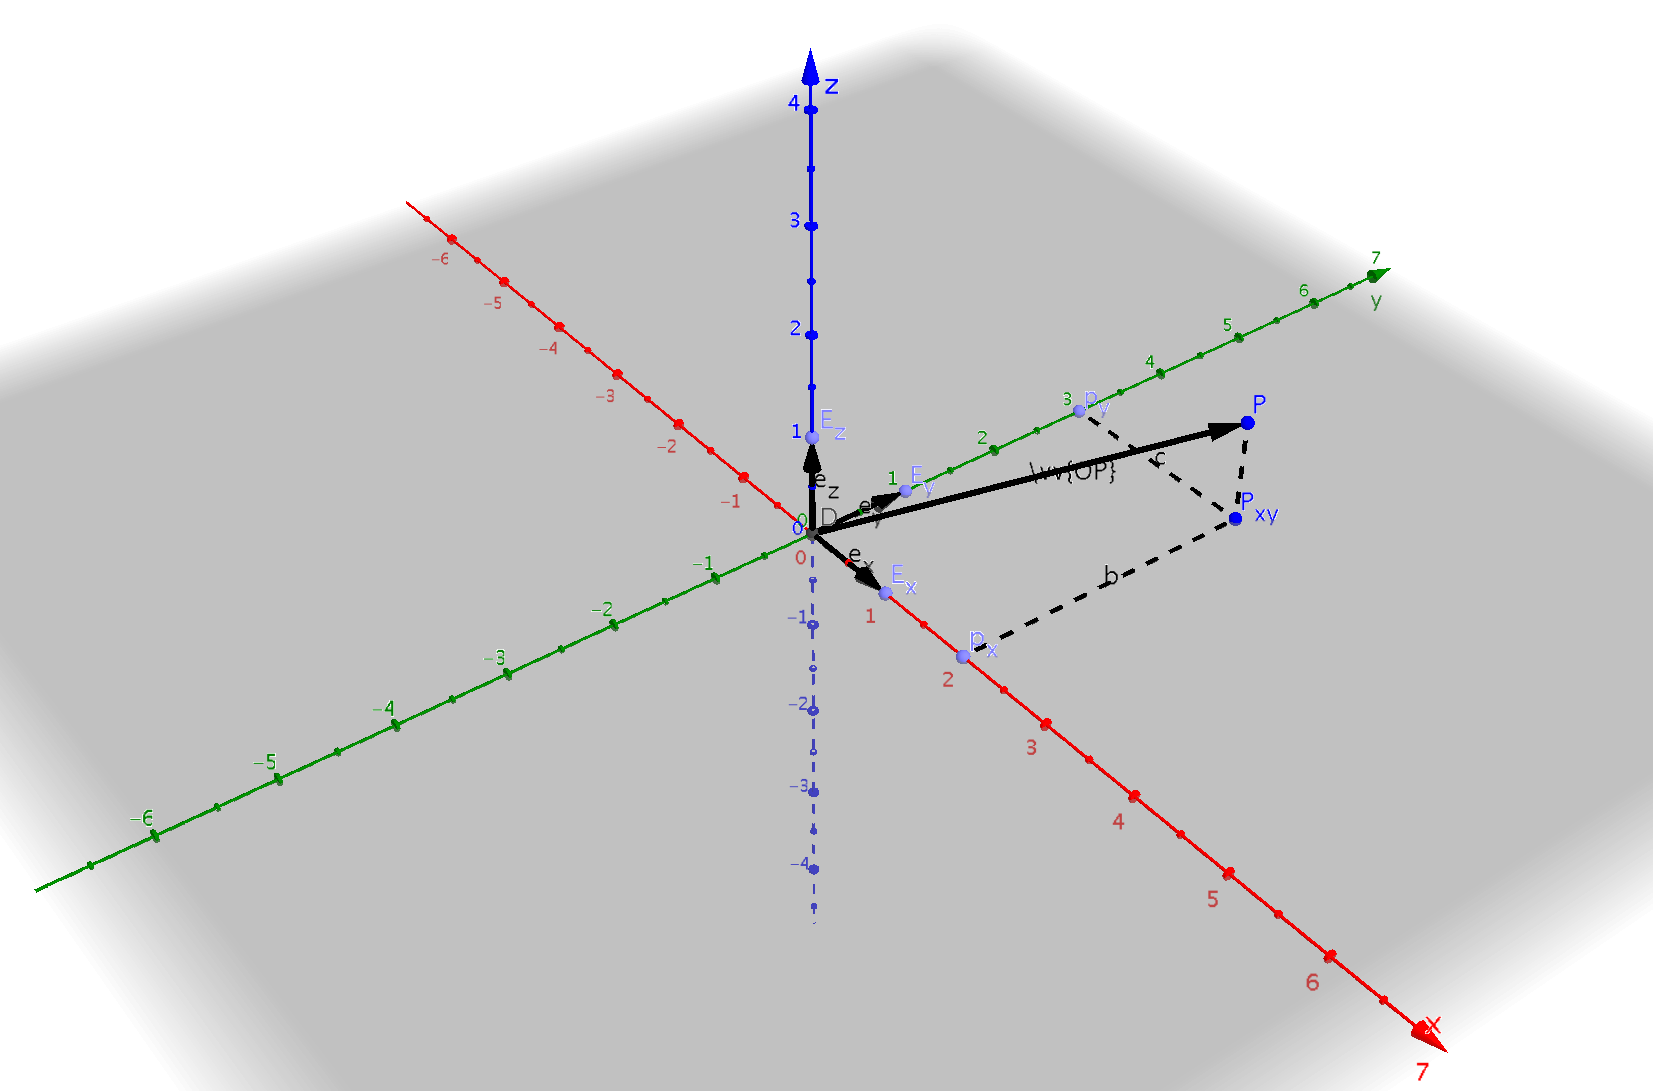
\includegraphics[width=10cm]{projektion.png}
\end{frame}

\subsubsection{Länge von Vektoren}
\begin{frame}{Länge eines Vektors 2-dimensional}
	Die Länge eines Vektors (seinen Betrag) kann man mit Hilfe des Satzes von Pythagoras bestimmen:
	\[
	\| \vv{a} \| = \sqrt{a_x^2 + a_y^2 } \qquad\text{für } \vv{a} = \begin{pmatrix}
	a_x \\ a_y
	\end{pmatrix}
	\]Also hier:	
	\[
	\| \vv{a} \| = \sqrt{3^2 + 4^2 } = \sqrt{9+16} = \sqrt{25} = 5 \qquad\text{für } \vv{a} = \begin{pmatrix}
	3 \\ 4
	\end{pmatrix}
	\]
%	\definecolor{ffzzqq}{rgb}{1.,0.6,0.}
\definecolor{ccwwqq}{rgb}{0.8,0.4,0.}
\definecolor{xdxdff}{rgb}{0.49019607843137253,0.49019607843137253,1.}
\definecolor{qqqqff}{rgb}{0.,0.,1.}
\definecolor{uuuuuu}{rgb}{0.26666666666666666,0.26666666666666666,0.26666666666666666}
\definecolor{cqcqcq}{rgb}{0.7529411764705882,0.7529411764705882,0.7529411764705882}
\begin{tikzpicture}[line cap=round,line join=round,>=triangle 45,x=1.0cm,y=1.0cm]
\draw [color=cqcqcq,, xstep=1.0cm,ystep=1.0cm] (-0.1303703703703693,-0.09925925925926203) grid (6.85037037037037,4.048888888888889);
\draw[->,color=black] (0.,0.) -- (6.85037037037037,0.);
\foreach \x in {,1.,2.,3.,4.,5.,6.}
\draw[shift={(\x,0)},color=black] (0pt,2pt) -- (0pt,-2pt) node[below] {\footnotesize $\x$};
\draw[->,color=black] (0.,0.) -- (0.,4.048888888888889);
\foreach \y in {,1.,2.,3.,4.}
\draw[shift={(0,\y)},color=black] (2pt,0pt) -- (-2pt,0pt) node[left] {\footnotesize $\y$};
\draw[color=black] (0pt,-10pt) node[right] {\footnotesize $0$};
\clip(-0.1303703703703693,-0.09925925925926203) rectangle (6.85037037037037,4.048888888888889);
\draw [->,line width=2.8pt] (0.,0.) -- (3.,4.);
\draw [line width=2.8pt,color=ccwwqq] (3.,4.)-- (3.,0.);
\draw [line width=2.8pt,color=ffzzqq] (3.,0.)-- (0.,0.);
\begin{scriptsize}
\draw [fill=uuuuuu] (0.,0.) circle (1.5pt);
\draw[color=uuuuuu] (0.04148148148148249,0.08444444444444182) node {$O$};
\draw [fill=qqqqff] (3.,4.) circle (1.5pt);
\draw[color=qqqqff] (3.04,4.001481481481482) node {$A$};
\draw[color=black] (2.0,2.0) node {$\vv{a}$};
\draw[color=black] (0.8,2.0) node {$\| \vv{a}\| = 5$};
\draw [fill=xdxdff] (3.,0.) circle (1.5pt);
\draw[color=xdxdff] (3.04,0.08444444444444182) node {$B$};
\draw[color=ccwwqq] (4.0044444444444447,2.0696296296296284) node {$a_y = 4$};
\draw[color=ffzzqq] (1.6,0.26148148148147892) node {$a_x = 3$};
\end{scriptsize}
\end{tikzpicture}
\definecolor{ffzzqq}{rgb}{1.,0.6,0.}
\definecolor{ccwwqq}{rgb}{0.8,0.4,0.}
\definecolor{xdxdff}{rgb}{0.49019607843137253,0.49019607843137253,1.}
\definecolor{qqqqff}{rgb}{0.,0.,1.}
\definecolor{uuuuuu}{rgb}{0.26666666666666666,0.26666666666666666,0.26666666666666666}
\definecolor{cqcqcq}{rgb}{0.7529411764705882,0.7529411764705882,0.7529411764705882}
\begin{tikzpicture}[line cap=round,line join=round,>=triangle 45,x=1.0cm,y=1.0cm]
\draw [color=cqcqcq,, xstep=1.0cm,ystep=1.0cm] (-0.1303703703703693,-0.09925925925926203) grid (6.85037037037037,4.048888888888889);
\draw[->,color=black] (0.,0.) -- (6.85037037037037,0.);
\foreach \x in {,1.,2.,3.,4.,5.,6.}
\draw[shift={(\x,0)},color=black] (0pt,2pt) -- (0pt,-2pt) node[below] {\footnotesize $\x$};
\draw[->,color=black] (0.,0.) -- (0.,4.048888888888889);
\foreach \y in {,1.,2.,3.,4.}
\draw[shift={(0,\y)},color=black] (2pt,0pt) -- (-2pt,0pt) node[left] {\footnotesize $\y$};
\draw[color=black] (0pt,-10pt) node[right] {\footnotesize $0$};
\clip(-0.1303703703703693,-0.09925925925926203) rectangle (6.85037037037037,4.048888888888889);
\draw [->,line width=2.8pt] (0.,0.) -- (3.,4.);
\draw [line width=2.8pt,color=ccwwqq] (3.,4.)-- (3.,0.);
\draw [line width=2.8pt,color=ffzzqq] (3.,0.)-- (0.,0.);
\begin{scriptsize}
\draw [fill=uuuuuu] (0.,0.) circle (1.5pt);
\draw[color=uuuuuu] (0.04148148148148249,0.08444444444444182) node {$O$};
\draw [fill=qqqqff] (3.,4.) circle (1.5pt);
\draw[color=qqqqff] (3.04,4.001481481481482) node {$A$};
\draw[color=black] (2.0,2.0) node {$\vv{a}$};
\draw[color=black] (0.8,2.0) node {$\| \vv{a}\| = 5$};
\draw [fill=xdxdff] (3.,0.) circle (1.5pt);
\draw[color=xdxdff] (3.04,0.08444444444444182) node {$B$};
\draw[color=ccwwqq] (4.0044444444444447,2.0696296296296284) node {$a_y = 4$};
\draw[color=ffzzqq] (1.6,0.26148148148147892) node {$a_x = 3$};
\end{scriptsize}
\end{tikzpicture}	
\end{frame}

\begin{frame}{Länge eines Vektors 3-dimensional}
	Die Betrag eines dreidimensionalen Vektors kann man ebenfalls mit Hilfe des Satzes von Pythagoras bestimmen:
	\[
	\| \vv{a} \| = \sqrt{a_x^2 + a_y^2 + a_z^2} \qquad\text{für } \vv{a} = \begin{pmatrix}
	a_x \\ a_y \\ a_z
	\end{pmatrix}
	\]
\end{frame}
\begin{frame}{Länge eines Vektors 3-dimensional}		
	\[
	\| \vv{a} \| = \sqrt{3^2 + 4^2 + 5^2} = \sqrt{50} = 7.0710... \qquad\text{für } \vv{a} = \begin{pmatrix}
	3 \\ 4 \\ 5
	\end{pmatrix}
	\]
	denn $a_{xy} = \sqrt{3^2 + 4^2}$ und $\|\vv{a}\| = \sqrt{a_{xy}^2 + a_z^2}$
	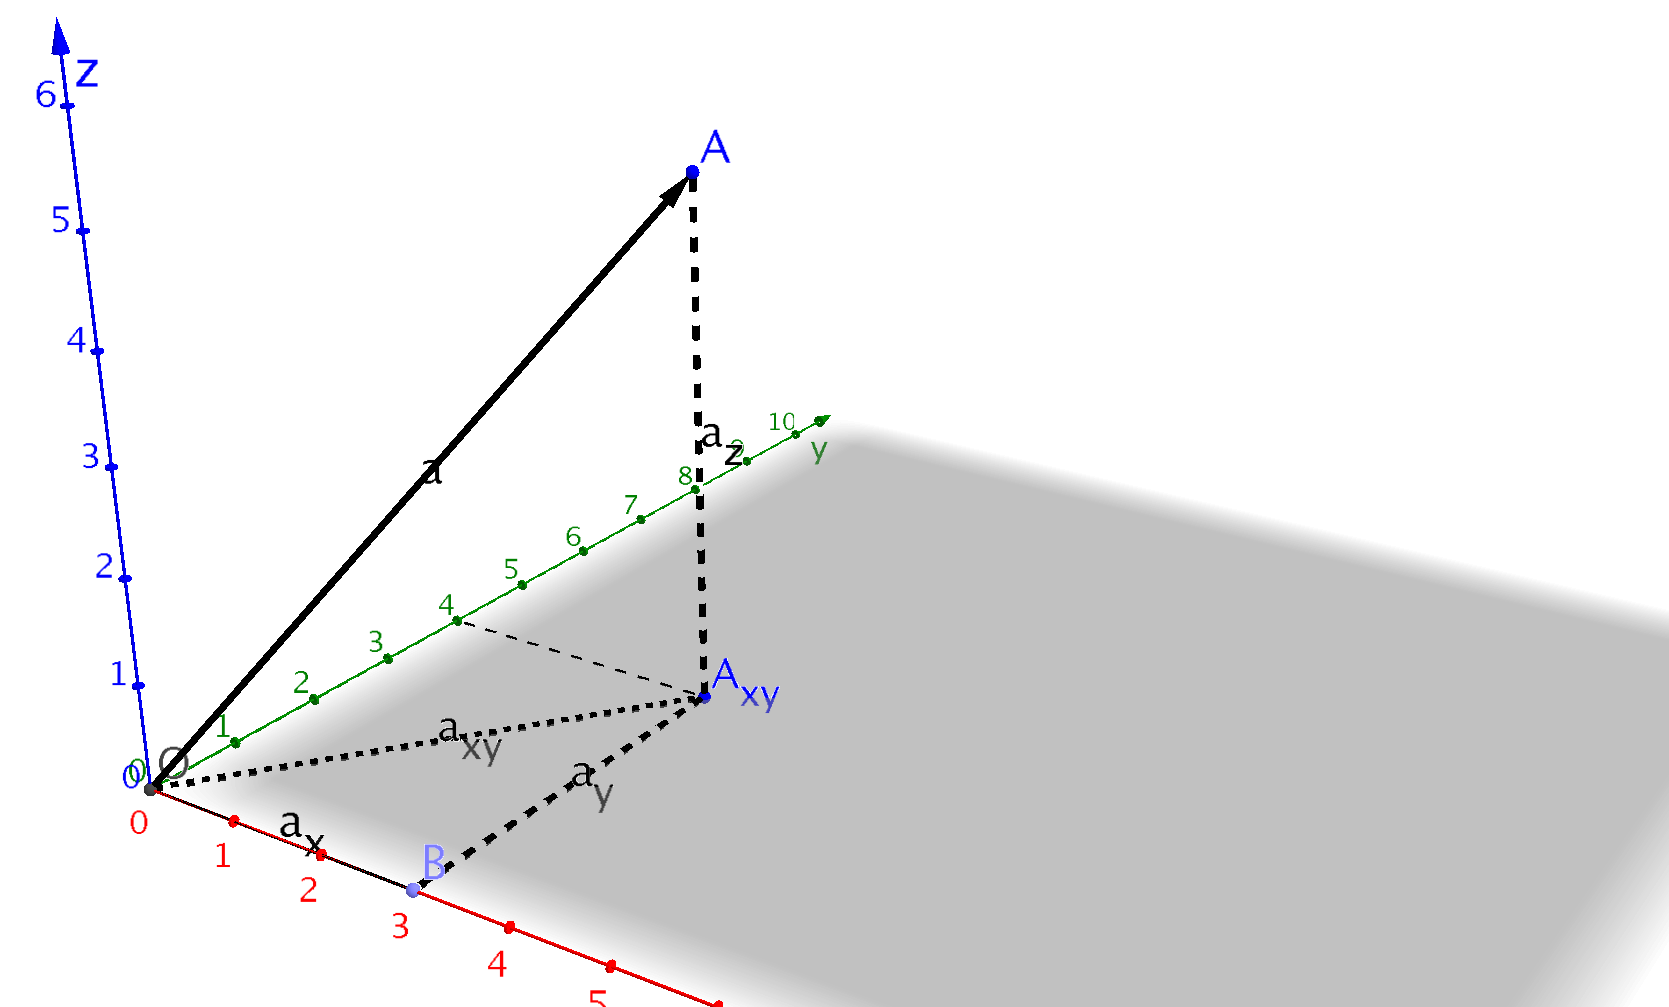
\includegraphics[width=10cm]{laengevektor3d.png}	
\end{frame}

\begin{frame}{Länge eines Vektors n-dimensional}
	Entsprechend gilt für die Länge n-dimensionaler Vektoren
	\[
	\| \vv{a} \| := \sqrt{a_1^2 + a_2^2 + \ldots + a_n^2}
	\]	
\end{frame}

\subsubsection{Skalarprodukt}
\begin{frame}{Produkte von Vektoren}
	Es gibt auch Produkte, an denen zwei Vektoren oder drei Vektoren beteiligt sind:
	\begin{itemize}
		\item \textbf{Skalarprodukt}
		
		 $\vv{a} \cdot \vv{b} \in \mathbb{R}$
		
		Das Ergebnis ist ein Skalar, also eine reelle Zahl
		\item \textbf{Vektor}- oder \textbf{Kreuzprodukt}
		
		$\vv{a} \times \vv{b} \in \mathbb{R}^3$
		
		Das Ergebnis ist ein (3-dimensionaler) Vektor.
		\item \textbf{Spatprodukt}
		
		$\left< \vv{a}, \vv{b}, \vv{c} \right> := \vv{a} \cdot (\vv{b} \times \vv{c} ) \in \mathbb{R}$
		
		Das Ergebnis ist eine Zahl, die das Volumen des von den drei Vektoren aufgespannten Spates ergibt.
	\end{itemize}	
\end{frame}


\begin{frame}{Skalarprodukt}
	\begin{definition}[Skalarprodukt]
		Das Skalarprodukt zweier Vektoren $\vv{a}$ und $\vv{b}$ ist definiert als
		\[
		\vv{a} \cdot \vv{b} := \begin{pmatrix}
		a_1 \\ a_2 \\ \vdots \\ a_n
		\end{pmatrix} \cdot
		\begin{pmatrix}
		b_1 \\ b_2 \\ \vdots \\ b_n
		\end{pmatrix} := a_1 b_1 + a_2 b_2  + \ldots + a_n b_n
		\]
	\end{definition}
	\begin{bemerkung}
		Die Komponenten werden also paarweise multipliziert und die Produkte addiert.
	\end{bemerkung}
\end{frame}

\begin{frame}{Skalarprodukt - Geometrische Bedeutung}
\begin{theorem}
	Für den zwischen zwei Vektoren $\vv{a}$ und $\vv{b}$ eingeschlossenen Winkel $\alpha$ gilt:
	\[
	\vv{a} \cdot \vv{b} = \| \vv{a} \| \| \vv{b} \| \cos \alpha
 \iff \cos \alpha = \frac{\vv{a}\cdot \vv{b}}{\| \vv{a} \| \| \vv{b} \| }	\]
	wobei $0 \leq \alpha \leq 180^\circ$.
\end{theorem}
\definecolor{qqwuqq}{rgb}{0.,0.39215686274509803,0.}
\definecolor{qqqqff}{rgb}{0.,0.,1.}
\definecolor{uuuuuu}{rgb}{0.26666666666666666,0.26666666666666666,0.26666666666666666}
\definecolor{cqcqcq}{rgb}{0.7529411764705882,0.7529411764705882,0.7529411764705882}
\begin{tikzpicture}[line cap=round,line join=round,>=triangle 45,x=1.0cm,y=1.0cm]
\draw [color=cqcqcq,, xstep=1.0cm,ystep=1.0cm] (-0.22494,-0.1387654320987674) grid (4.428888888888889,2.6266666666666683);
\draw[->,color=black] (-0.22494,0.) -- (4.428888888888889,0.);
\foreach \x in {,1.,2.,3.,4.}
\draw[shift={(\x,0)},color=black] (0pt,2pt) -- (0pt,-2pt) node[below] {\footnotesize $\x$};
\draw[->,color=black] (0.,-0.1387654320987674) -- (0.,2.6266666666666683);
\foreach \y in {,1.,2.}
\draw[shift={(0,\y)},color=black] (2pt,0pt) -- (-2pt,0pt) node[left] {\footnotesize $\y$};
\draw[color=black] (0pt,-10pt) node[right] {\footnotesize $0$};
\clip(-0.22494,-0.1387654320987674) rectangle (4.428888888888889,2.6266666666666683);
\draw [shift={(0.,0.)},color=qqwuqq,fill=green,fill opacity=2] (0,0) -- (0.:1) arc (0.:63.43494882292201:1) -- cycle;
\draw [->,line width=2.pt] (0.,0.) -- (1.,2.);
\draw [->,line width=2.pt] (0.,0.) -- (2.,0.);
\begin{scriptsize}
\draw [fill=uuuuuu] (0.,0.) circle (1.5pt);
\draw [fill=qqqqff] (1.,2.) circle (1.5pt);
\draw[color=qqqqff] (1.0274061441237503,2.053827160493828) node {$B$};
\draw[color=black] (0.4940726127145822,1.0424691358024687) node {$a$};
\draw [fill=qqqqff] (2.,0.) circle (1.5pt);
\draw[color=qqqqff] (2.026912688172043,0.054814814814813095) node {$C$};
\draw[color=black] (1.0116036691190342,0.050864197530862465) node {$b$};
\draw[color=qqwuqq] (1.22147991888322963,0.250864197530862465) node {$\alpha = 63.43\textrm{\degre}$};
\end{scriptsize}
\end{tikzpicture}

Insbesondere ist
	$
	\| \vv{a} \| = \sqrt{ \vv{a} \cdot \vv{a} }
	$
\end{frame}



\begin{frame}{Skalarprodukt - Rechenregeln}
	\begin{theorem}	
		Für das Skalarprodukt gilt \textbf{das Kommutativ-Gesetz}
		\[
			\vv{a} \cdot \vv{b} = \vv{b} \cdot \vv{a}
		\]
		als auch \textbf{das Distributiv-Gesetz}
		\[
			\vv{a} \cdot \left( \vv{b} + \vv{c} \right) = \vv{a} \cdot \vv{b} + \vv{a} \cdot \vv{c} \mbox{ und } \left( \lambda \vv{a} \right) \cdot \vv{b} = \lambda \left( \vv{a} \cdot \vv{b} \right)
 		\]
		
		Zudem sind zwei Vektoren $\vv{a}$ und $\vv{b}$ senkrecht aufeinander genau dann, wenn $\vv{a}\cdot\vv{b}=0$:
		\[
		\vv{a} \perp \vv{b} \Leftrightarrow \vv{a} \cdot \vv{b} = 0
		\]
	\end{theorem}	
\end{frame}

\begin{frame}{Kosinussatz}
	\begin{theorem}
		Für zwei Vektoren $\vv{a}$ und $\vv{b}$ gilt:
		\[
		\| \vv{a} - \vv{b}\|^2 = \|\vv{a}\|^2 + \|\vv{b}\|^2 - 2 \vv{a} \cdot \vv{b}
		\]
	\end{theorem}
	\begin{bemerkung}
		Dieser Satz ist der aus der Schule bekannte Kosinussatz:
		\[
			c^2 = a^2 + b^2 - 2 a b \cos \gamma
		\]
		wobei $\gamma$ der Winkel zwischen den Seiten $a$ und $b$ ist, denn
		\[
		\vv{a} \cdot \vv{b} = \| \vv{a} \| \| \vv{b} \| \cos \gamma
		\]
		Für $\vv{a} \perp \vv{b}$ ist das der Satz des Pythagoras:
		\[
			\left\| \vv{a} - \vv{b} \right\|^2 = \|\vv{a}\|^2 + \|\vv{b}\|^2
		\]
	\end{bemerkung}
\end{frame}

\begin{frame}{Cauchy-Schwarzsche Ungleichung}
	\begin{theorem}
		Für das Skalarprodukt gilt die Ungleichung:
		\[
			| \vv{a} \cdot \vv{b} | \leq \|\vv{a}\| \|\vv{b}\|
		\]
		für beliebige Vektoren $\vv{a}$ und $\vv{b}$.
	\end{theorem}
	Irgendwie klar, weil $|\cos \gamma| \leq 1$ für beliebige Winkel $\gamma$.
\end{frame}

\begin{frame}{Skalarprodukt - Anwendungsbeispiel}
	Greift eine konstante Kraft $\vv{F}$  an einem Massepunkt $M$ an und verschiebt ihn dabei um die Strecke $\vv{s}$, so gilt für die am Massepunkt $M$ geleistete Arbeit $W$ (das ist ein Skalar!)
	\[
		W = \vv{F} \cdot \vv{s} = \| \vv{F} \| \| \vv{s} \| \cos \alpha = \| \vv{F_s}\| \|\vv{s}\|
	\]
	wobei $\alpha$ der Winkel zwischen der Richtung der Kraft $\vv{F}$ und der Bewegungsrichtung $\vv{s}$ und $\vv{F_s} := \frac{\vv{F} \cdot \vv{s}}{\|\vv{s}\|} \frac{\vv{s}}{\|\vv{s}\|} = \left(\vv{F} \cdot \vv{e_s} \right) \vv{e_s}$ ist.
\definecolor{ffzztt}{rgb}{1.,0.6,0.2}
\definecolor{qqwuqq}{rgb}{0.,0.39215686274509803,0.}
\definecolor{ffqqtt}{rgb}{1.,0.,0.2}
\definecolor{qqqqff}{rgb}{0.,0.,1.}
\begin{tikzpicture}[line cap=round,line join=round,>=triangle 45,x=1.2cm,y=1.2cm]
\clip(0.9985185185185195,1.4340740740740714) rectangle (8.305185185185188,5.582222222222217);
\draw [shift={(2.,2.)},color=yellow,fill=green,fill opacity=0.1] (0,0) -- (0.:0.5777777777777778) arc (0.:36.86989764584402:0.5777777777777778) -- cycle;
\draw [->,color=ffqqtt] (2.,2.) -- (4.,2.);
\draw [->] (2.,2.) -- (6.,5.);
\draw [line width=1.pt,dotted] (6.,5.)-- (6.,2.);
\draw [->,color=ffzztt] (2.,2.) -- (6.,2.);
\begin{scriptsize}
\draw [fill=qqqqff] (2.,2.) circle (0.5pt);
\draw[color=qqqqff] (2.0414814814814823,2.285925925925923) node {$M$};
\draw [fill=qqqqff] (6.,5.) circle (0.5pt);
\draw [fill=qqqqff] (4.,2.) circle (0.5pt);
\draw[color=ffqqtt] (3.0133333333333345,2.1740740740740713) node {$\vv{s}$};
\draw[color=black] (4.002962962962964,3.767407407407404) node {$\vv{F}$};
\draw[color=qqwuqq] (2.3837037037037046,2.1562962962962934) node {$\alpha$};
\draw [fill=qqqqff] (6.,2.) circle (0.5pt);
\draw[color=ffzztt] (4.026666666666667,2.2918518518518487) node {$\vv{F_s}$};
\end{scriptsize}
\end{tikzpicture}
\end{frame}

\subsubsection{Vektorprodukt}
\begin{frame}{Vektorprodukt / Kreuzprodukt / äußeres Produkt}
	Für zwei \textbf{dreidimensionale} Vektoren
	\[
	\vv{a} = \begin{pmatrix}
	a_x \\ a_y \\ a_z
	\end{pmatrix} \mbox{ und } 	\vv{b} = \begin{pmatrix}
	b_x \\ b_y \\ b_z
	\end{pmatrix}
 	\]
 	ist das \textbf{Kreuzprodukt} (auch \textbf{Vektorprodukt} oder \textbf{äußeres Produkt}) definiert als
 	\[
	 	\vv{a} \times \vv{b} := \begin{pmatrix}
	 	a_y b_z - a_z b_y \\
	 	a_z b_x - a_x b_z \\
	 	a_x b_y - a_y b_x
	 	\end{pmatrix} \in \mathbb{R}^3
 	\]
\end{frame}

\begin{frame}{Eigenschaften des Vektorproduktes}
	Für beliebige Vektoren $\vv{a} \in \mathbb{R}^3$, $\vv{b} \in \mathbb{R}^3$ und $\vv{c} \in \mathbb{R}^3$ und beliebiges $\lambda \in \mathbb{R}$ gilt:
	\[	\vv{a}, \vv{b} \mbox{ und } \vv{a}  \times  		\vv{b}  \mbox{ bilden ein Rechts-System}
	\]
	\begin{align*}
		\vv{a} \times \vv{b} & =  - \vv{b} \times \vv{a} \\
		\left( \lambda \vv{a} \right) \times \vv{b} & =  \vv{a} \times \left( \lambda \vv{b} \right) = \lambda \left( \vv{a} \times \vv{b} \right)  \\
		\vv{a} \times \left( \vv{b} + \vv{c} \right) & =   \vv{a} \times \vv{b} + \vv{a} \times \vv{c} \\
		\vv{a} \times \vv{b} = \vv{0} &  \Leftrightarrow  \vv{a} \| \vv{b}  \\
		\left(\vv{a} \times \vv{b}\right) \perp \vv{a} & \mbox{ und }  \left(\vv{a} \times \vv{b}\right) \perp \vv{b} \\
		\left\| \vv{a} \times \vv{b} \right\| & =  \|\vv{a}\| \|\vv{b}\| \sin \alpha
	\end{align*}
	wobei $0 \leq \alpha \leq 180^\circ$ der von $\vv{a}$ und $\vv{b}$ eingeschlossene Winkel ist.
\end{frame}

\begin{frame}{Kreuzprodukt - Beispiel}
	
	\begin{align*}
	\begin{pmatrix}
	1 \\ 0 \\ 0
	\end{pmatrix} \times  \begin{pmatrix}
	0 \\ 1 \\ 0
	\end{pmatrix} & = \begin{pmatrix}
	0 \cdot 0 - 0 \cdot 1 \\
	0 \cdot 0 - 1 \cdot 0 \\
	1 \cdot 1 - 0 \cdot 0	
	\end{pmatrix} = \begin{pmatrix}
	0 \\ 0 \\ 1
	\end{pmatrix} \\
	\begin{pmatrix}
	1 \\ 0 \\ 0
	\end{pmatrix} \times  \begin{pmatrix}
	1 \\ 1 \\ 0
	\end{pmatrix} & = \begin{pmatrix}
	0 \cdot 0 - 0 \cdot 1 \\
	0 \cdot 1 - 1 \cdot 0 \\
	1 \cdot 1 - 0 \cdot 1	
	\end{pmatrix} = \begin{pmatrix}
	0 \\ 0 \\ 1
	\end{pmatrix} \\
	\begin{pmatrix}
		1 \\ 0 \\ 3
	\end{pmatrix} \times  \begin{pmatrix}
	2 \\ -3 \\ 4
	\end{pmatrix} & = \begin{pmatrix}
	0 \cdot 4 - 3 \cdot (-3) \\
	3 \cdot 2 - 1 \cdot 4 \\
	1 \cdot -3 - 0 \cdot 2	
	\end{pmatrix} = \begin{pmatrix}
	9 \\ 2 \\ -3
	\end{pmatrix}
	\end{align*}
{\scriptsize 	%\href{/Users/stefan/sciebo/Mathematik/EigeneVorlesung/Folien/kreuzprodukt.ggb}{Beispiel Kreuzprodukt Geogebra}
\href{https://fh-swf.sciebo.de/public.php?service=files&t=83c3e87e19f49991d0d6c55da10f8c7d}{Beispiel Kreuzprodukt Geogebra}
}\end{frame}

\begin{frame}{Kreuzprodukt - Anwendungen}
	Das von zwei Vektoren $\vv{a}$ und $\vv{b}$ aufgespannte Parallelogramm hat den Flächeninhalt
	\[
		\| \vv{a} \times \vv{b}\| = \left|  \|\vv{a}\| \|\vv{b}\| \sin \alpha \right|
	\]
	\href{/Users/stefan/sciebo/Mathematik/EigeneVorlesung/Folien/parallelogramm.ggb}{Parallelogramm-Beispiel}
	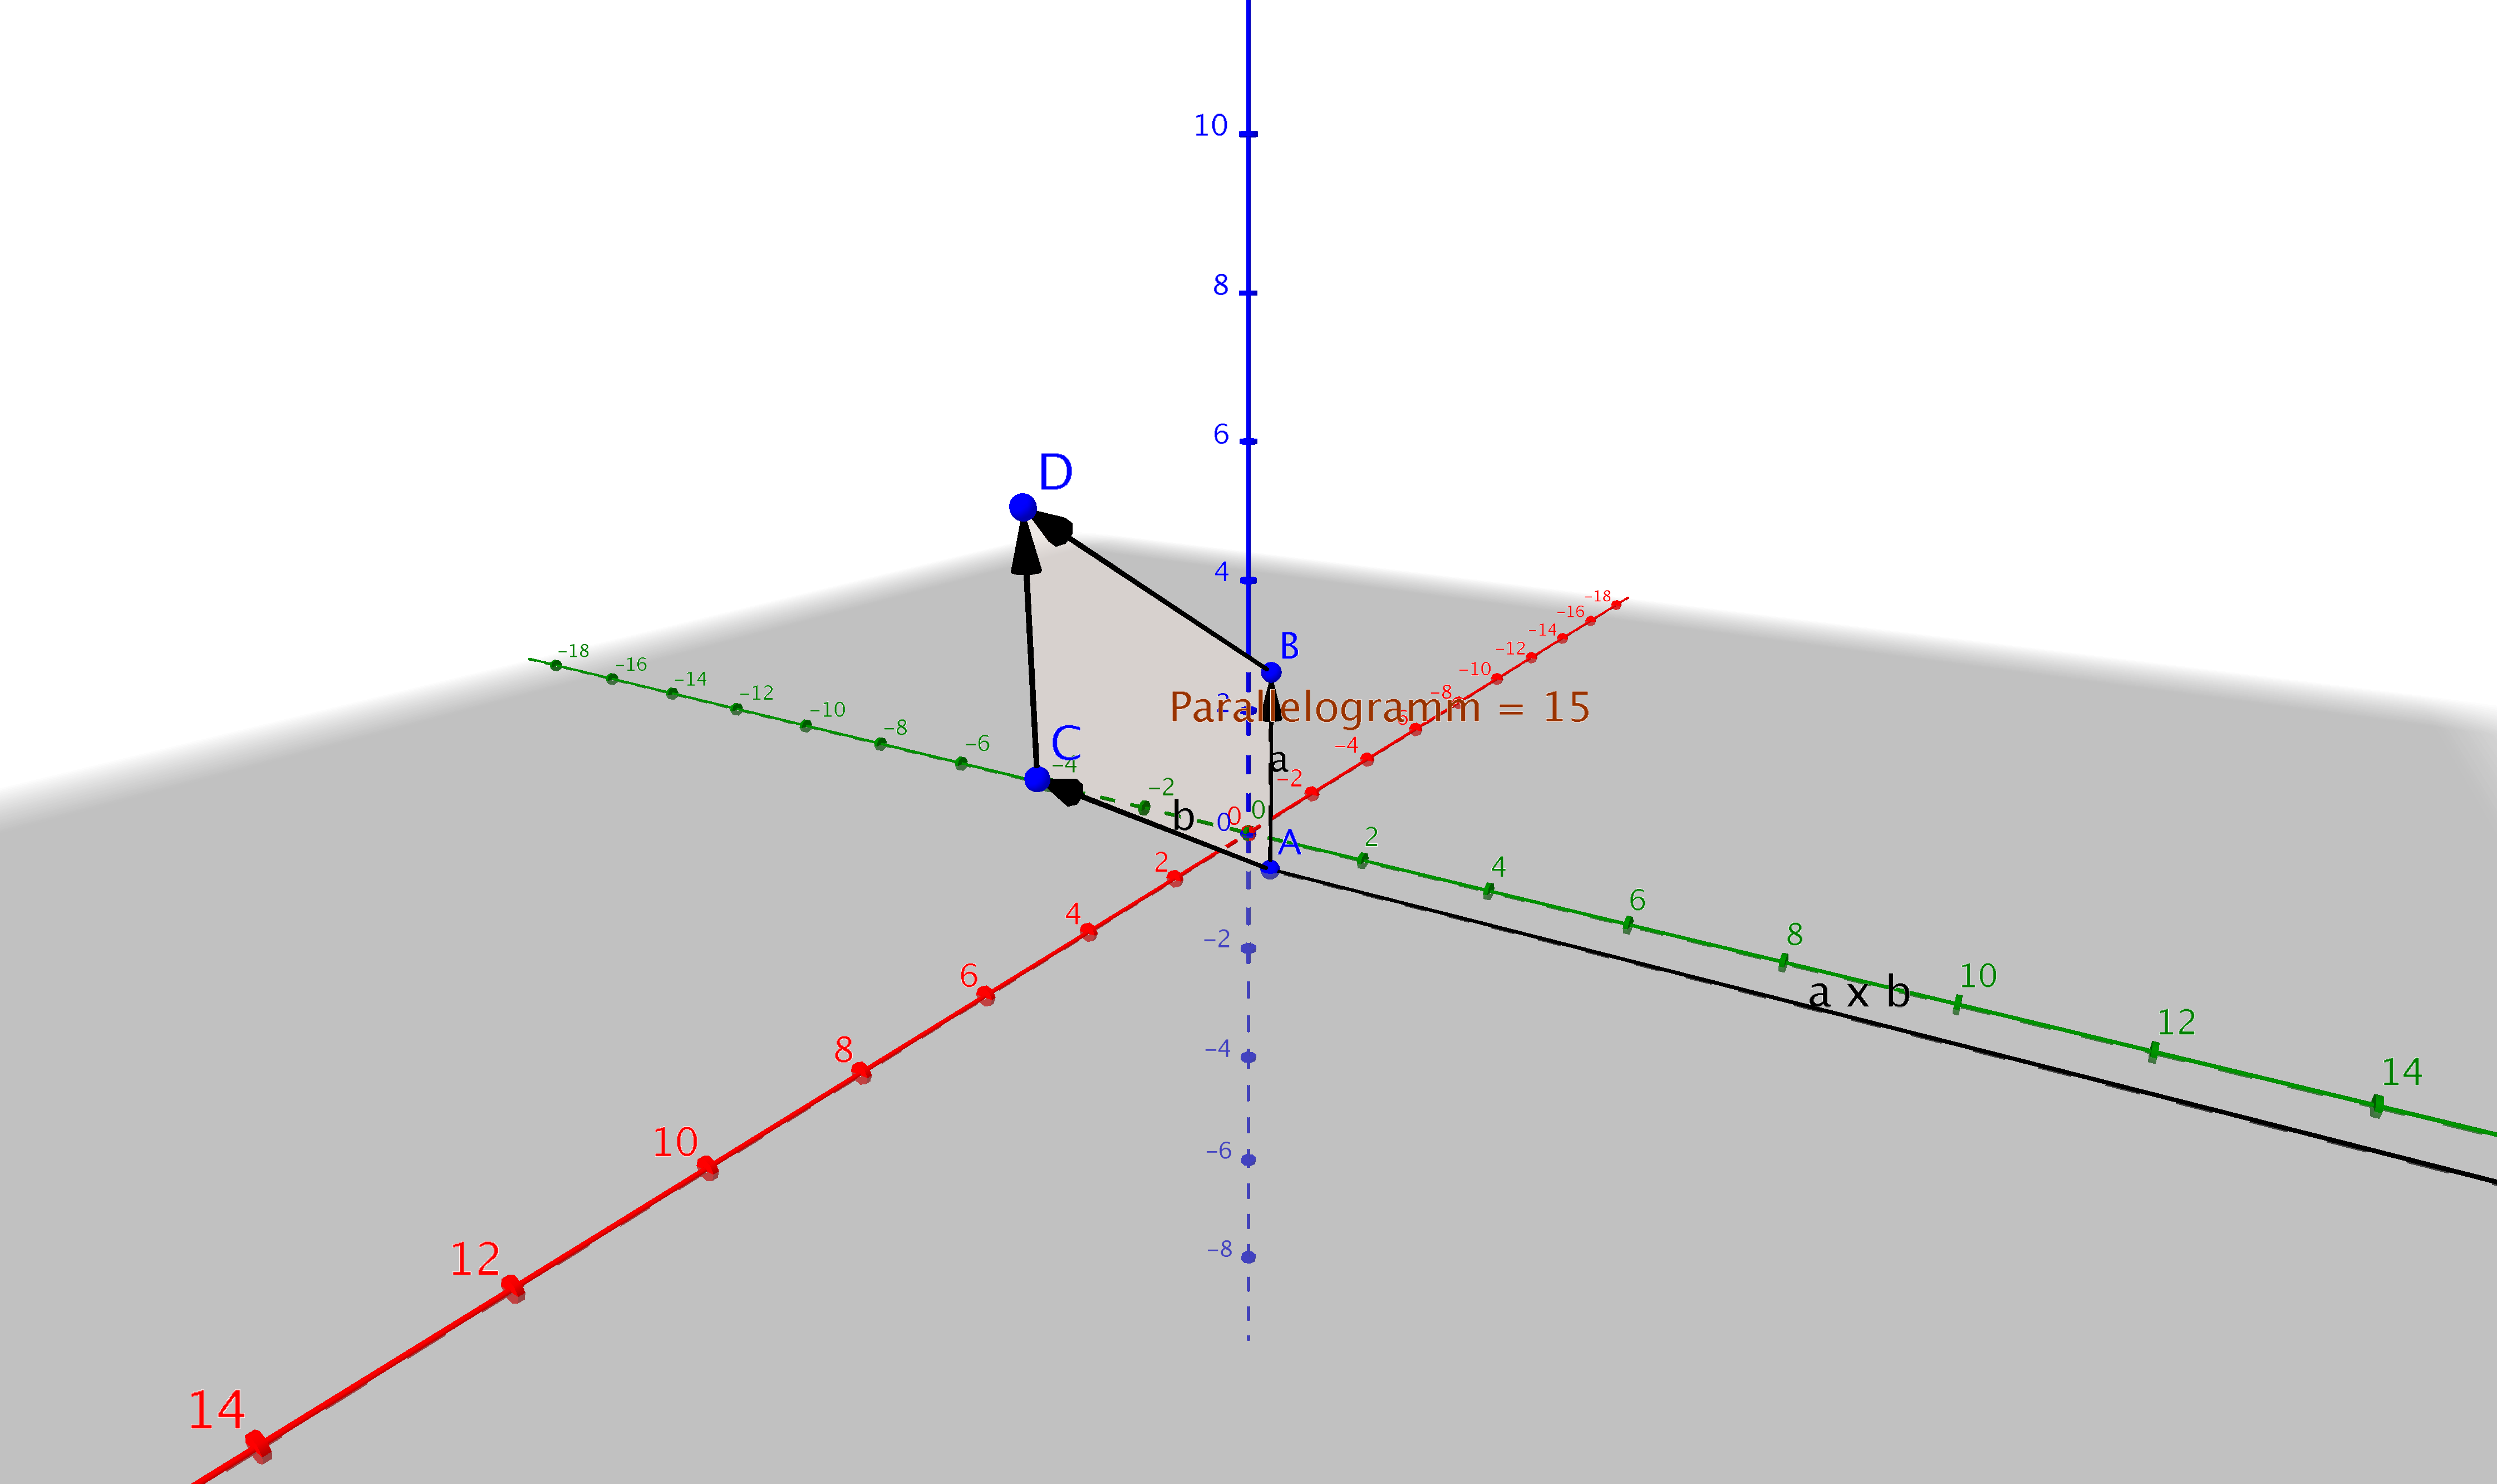
\includegraphics[width=10cm]{parallelogramm.png}
\end{frame}

\begin{frame}{Kreuzprodukt - Drehmoment}
	Greift eine Kraft $\vv{F}$ am Rand einer drehbar  gelagerten Kreisscheibe mit dem Ortsvektor $\vv{r}$ an, so wirkt auf die Scheibe das Drehmoment
	\[
		\vv{M} = \vv{r} \times \vv{F}
	\]
	mit
	\[
		\| \vv{M} \| = \| \vv{r}\| \|\vv{F}\| \sin \alpha
	\]
\definecolor{qqwuqq}{rgb}{0.,0.39215686274509803,0.}
\definecolor{uuuuuu}{rgb}{0.26666666666666666,0.26666666666666666,0.26666666666666666}
\definecolor{xdxdff}{rgb}{0.49019607843137253,0.49019607843137253,1.}
\definecolor{qqqqff}{rgb}{0.,0.,1.}
\begin{tikzpicture}[line cap=round,line join=round,>=triangle 45,x=0.9cm,y=0.9cm]
\draw[->,color=black] (-1.6177777777777769,0.) -- (8.853333333333339,0.);
\foreach \x in {-1.5,-1.,-0.5,0.5,1.,1.5,2.,2.5,3.,3.5,4.,4.5,5.,5.5,6.,6.5,7.,7.5,8.,8.5}
\draw[shift={(\x,0)},color=black] (0pt,2pt) -- (0pt,-2pt) node[below] {\footnotesize $\x$};
\draw[->,color=black] (0.,-0.18666666666666967) -- (0.,6.035555555555551);
\foreach \y in {,0.5,1.,1.5,2.,2.5,3.,3.5,4.,4.5,5.,5.5,6.}
\draw[shift={(0,\y)},color=black] (2pt,0pt) -- (-2pt,0pt) node[left] {\footnotesize $\y$};
\draw[color=black] (0pt,-10pt) node[right] {\footnotesize $0$};
\clip(-1.6177777777777769,-0.18666666666666967) rectangle (8.853333333333339,6.035555555555551);
\draw [shift={(3.7680568414275446,4.4236284792602305)},color=green,fill=green,fill opacity=0.1] (0,0) -- (-36.111057521575496:0.5666666666666668) arc (-36.111057521575496:8.623241639417227:0.5666666666666668) -- cycle;
\draw(2.,2.) circle (2.7cm);
\draw [->] (2.,2.) -- (3.7680568414275446,4.4236284792602305);
\draw [->] (3.7680568414275446,4.4236284792602305) -- (8.36,5.12);
\draw [->] (3.7680568414275446,4.4236284792602305) -- (6.43349336850494,2.479170684916884);
\draw [dash pattern=on 2pt off 2pt] (8.36,5.12)-- (6.43349336850494,2.479170684916884);
\begin{scriptsize}
\draw [fill=qqqqff] (2.,2.) circle (1.5pt);
\draw[color=qqqqff] (2.062222222222225,2.124444444444441) node {$M$};
%\draw[color=black] (0.5244444444444462,4.44444444444444) node {$???$};
\draw [fill=xdxdff] (3.7680568414275446,4.4236284792602305) circle (1.5pt);
\draw[color=xdxdff] (3.8311111111111145,4.551111111111107) node {$P$};
\draw[color=black] (2.88,3.306666666666663) node {$r$};
\draw [fill=qqqqff] (8.36,5.12) circle (1.5pt);
\draw[color=qqqqff] (8.417777777777784,5.24444444444444) node {$A$};
\draw[color=black] (6.08,4.88) node {$F$};
\draw [fill=uuuuuu] (6.43349336850494,2.479170684916884) circle (1.5pt);
\draw[color=uuuuuu] (6.497777777777782,2.604444444444441) node {$B$};
\draw[color=black] (5.351111111111115,3.555555555555552) node {$\vv{F}^{\perp}_{\vv{r}}$};
\draw[color=qqwuqq] (4.8933333333333366,4.357777777777774) node {$\alpha = 44.73\textrm{\degre}$};
\end{scriptsize}
\end{tikzpicture}	
\end{frame}

\subsubsection{Spatprodukt}
\begin{frame}{Spatprodukt}
	Ein durch drei Vektoren $\vv{a}, \vv{b}, \vv{c} \in \mathbb{R}^3$ aufgespanntes Parallelotop/Spat hat das Volumen
	\[
		V = \left| \vv{a} \cdot \left( \vv{b} \times \vv{c} \right) \right|
	\]
	\begin{definition}
		Der Ausdruck
		\[
			\left< \vv{a}, \vv{b}, \vv{c} \right> := \vv{a} \cdot \left( \vv{b} \times \vv{c} \right)
		\]
		heißt \textbf{Spatprodukt} der Vektoren $\vv{a}, \vv{b}, \vv{c}$
	\end{definition}
\end{frame}

\begin{frame}{Spatprodukt - Geometrie}
	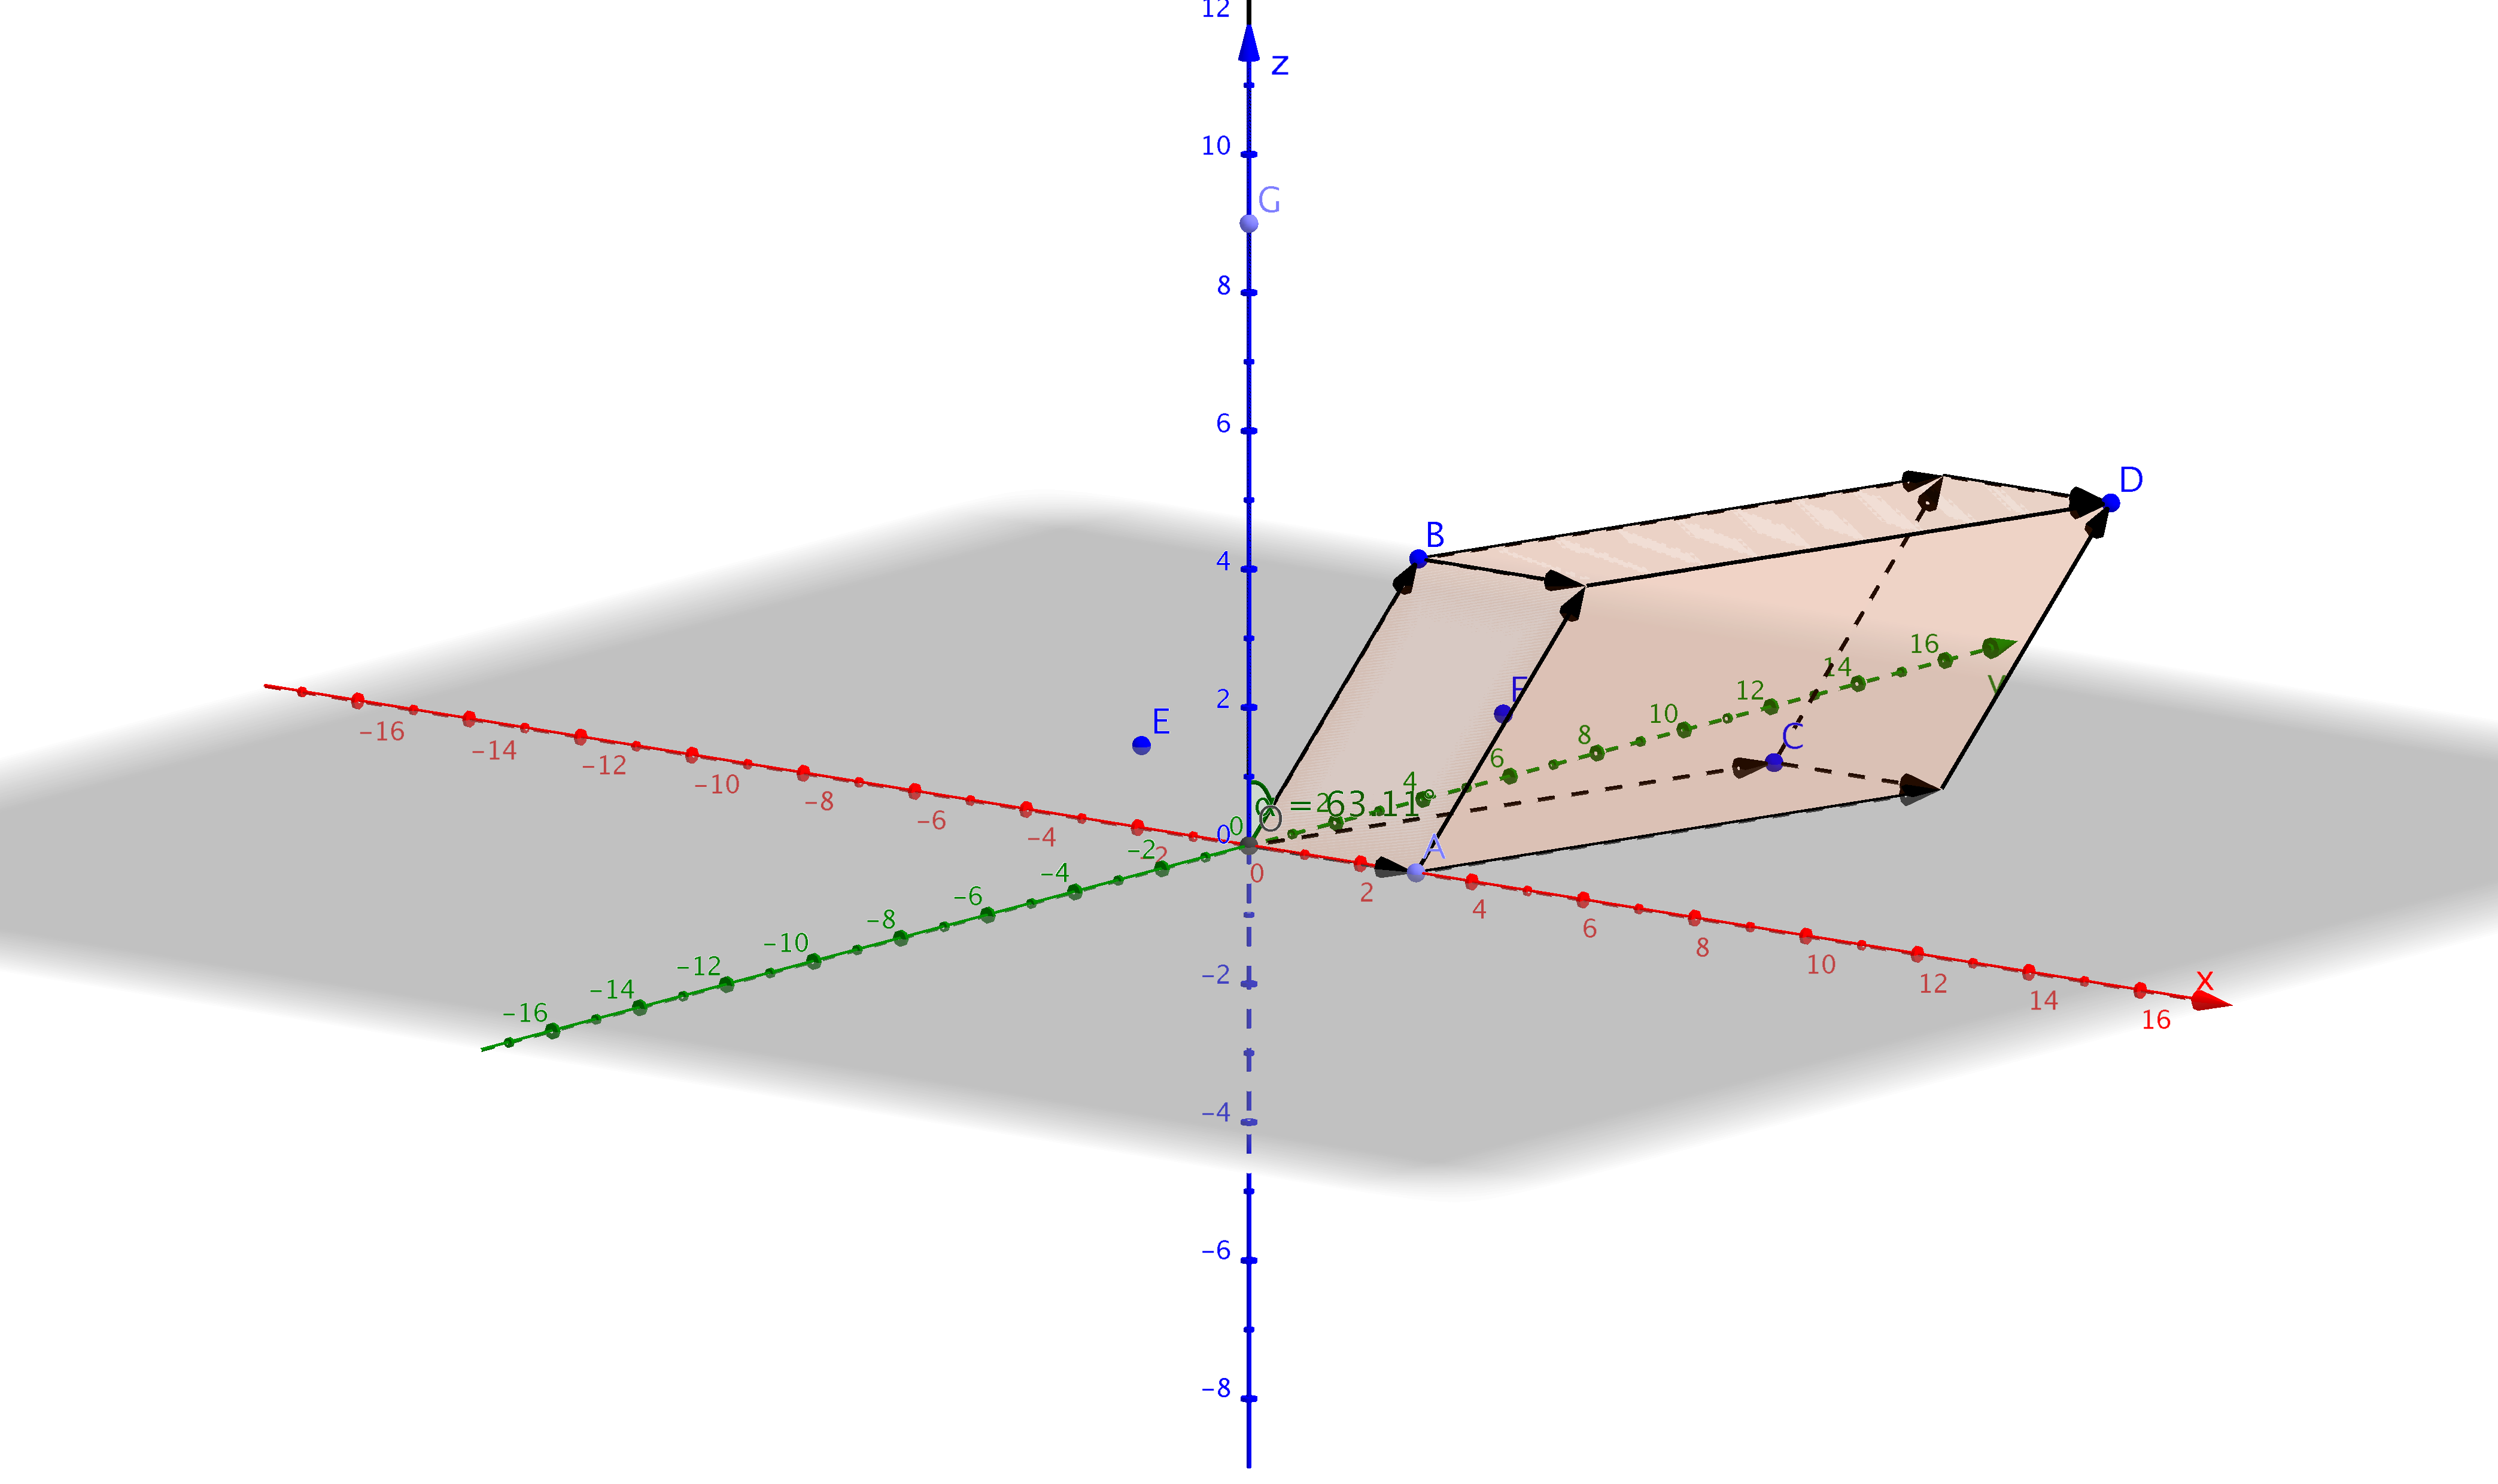
\includegraphics[width=10cm]{parallelotop.png}
	
	\href{/Users/stefan/sciebo/Mathematik/EigeneVorlesung/Folien/parallelotop.ggb}{Parallelotop Geogebra}
\end{frame}

\begin{frame}{Geraden - Parameterdarstellung}
	Eine Gerade ist durch die Angabe zweier Punkte auf ihr eindeutig bestimmt.
	
	Sind $A$ und $B$ zwei (verschiedene) Punkte einer Geraden und $\vv{a}$ und $\vv{b}$ die dazugehörigen Ortsvektoren,
	so kann man die Menge der Punkte der Geraden $g(A,B)$ durch $A$ und $B$ definieren als:
	\[
		g(A,B) := \left\{ \vv{y} \in \mathbb{R}^n \middle| \vv{y} = \vv{a} + \lambda \left( \vv{b} - \vv{a}\right), \lambda \in \mathbb{R}\right\}
	\]
	Diese Darstellung einer Geraden heißt \textbf{Parameterdarstellung der Geraden}. Der Parameter ist hier das $\lambda$.
\end{frame}

\subsection{Analytische Geometrie}
\subsubsection{Geraden}
\begin{frame}{Parameterdarstellung einer Gerade - Beispiel}
	Für die Punkte $A=\begin{pmatrix}
	3 \\ 4 \\ 1
	\end{pmatrix}$ und $B=\begin{pmatrix}
	2 \\ 4 \\ -1
	\end{pmatrix}$ ist
	\[
		g(A,B)  =  \left\{ \vv{y} \in \mathbb{R}^3 \middle| \vv{y} = \begin{pmatrix}
		3 \\ 4 \\ 1
		\end{pmatrix}
		 + \lambda \begin{pmatrix}
		 -1 \\ 0 \\ -2
		 \end{pmatrix}, \lambda \in \mathbb{R}\right\}
	\]
	Das ist z. B.
	\begin{itemize}
		\item für $\lambda = 0$ der Punkt $A$ mit dem Ortsvektor $\begin{pmatrix}
			3 \\ 4 \\ 1
		\end{pmatrix} $
		\item für $\lambda = 1$ der Punkt $B$ mit dem Ortsvektor $\begin{pmatrix}
			2 \\ 4 \\ -1
		\end{pmatrix}$
		\item und für $\lambda = 2$ der Punkt mit dem Ortsvektor $\begin{pmatrix}
			1 \\ 4 \\ -3
		\end{pmatrix}$
	\end{itemize}
\end{frame}

\begin{frame}{Parameterdarstellung einer Gerade}
	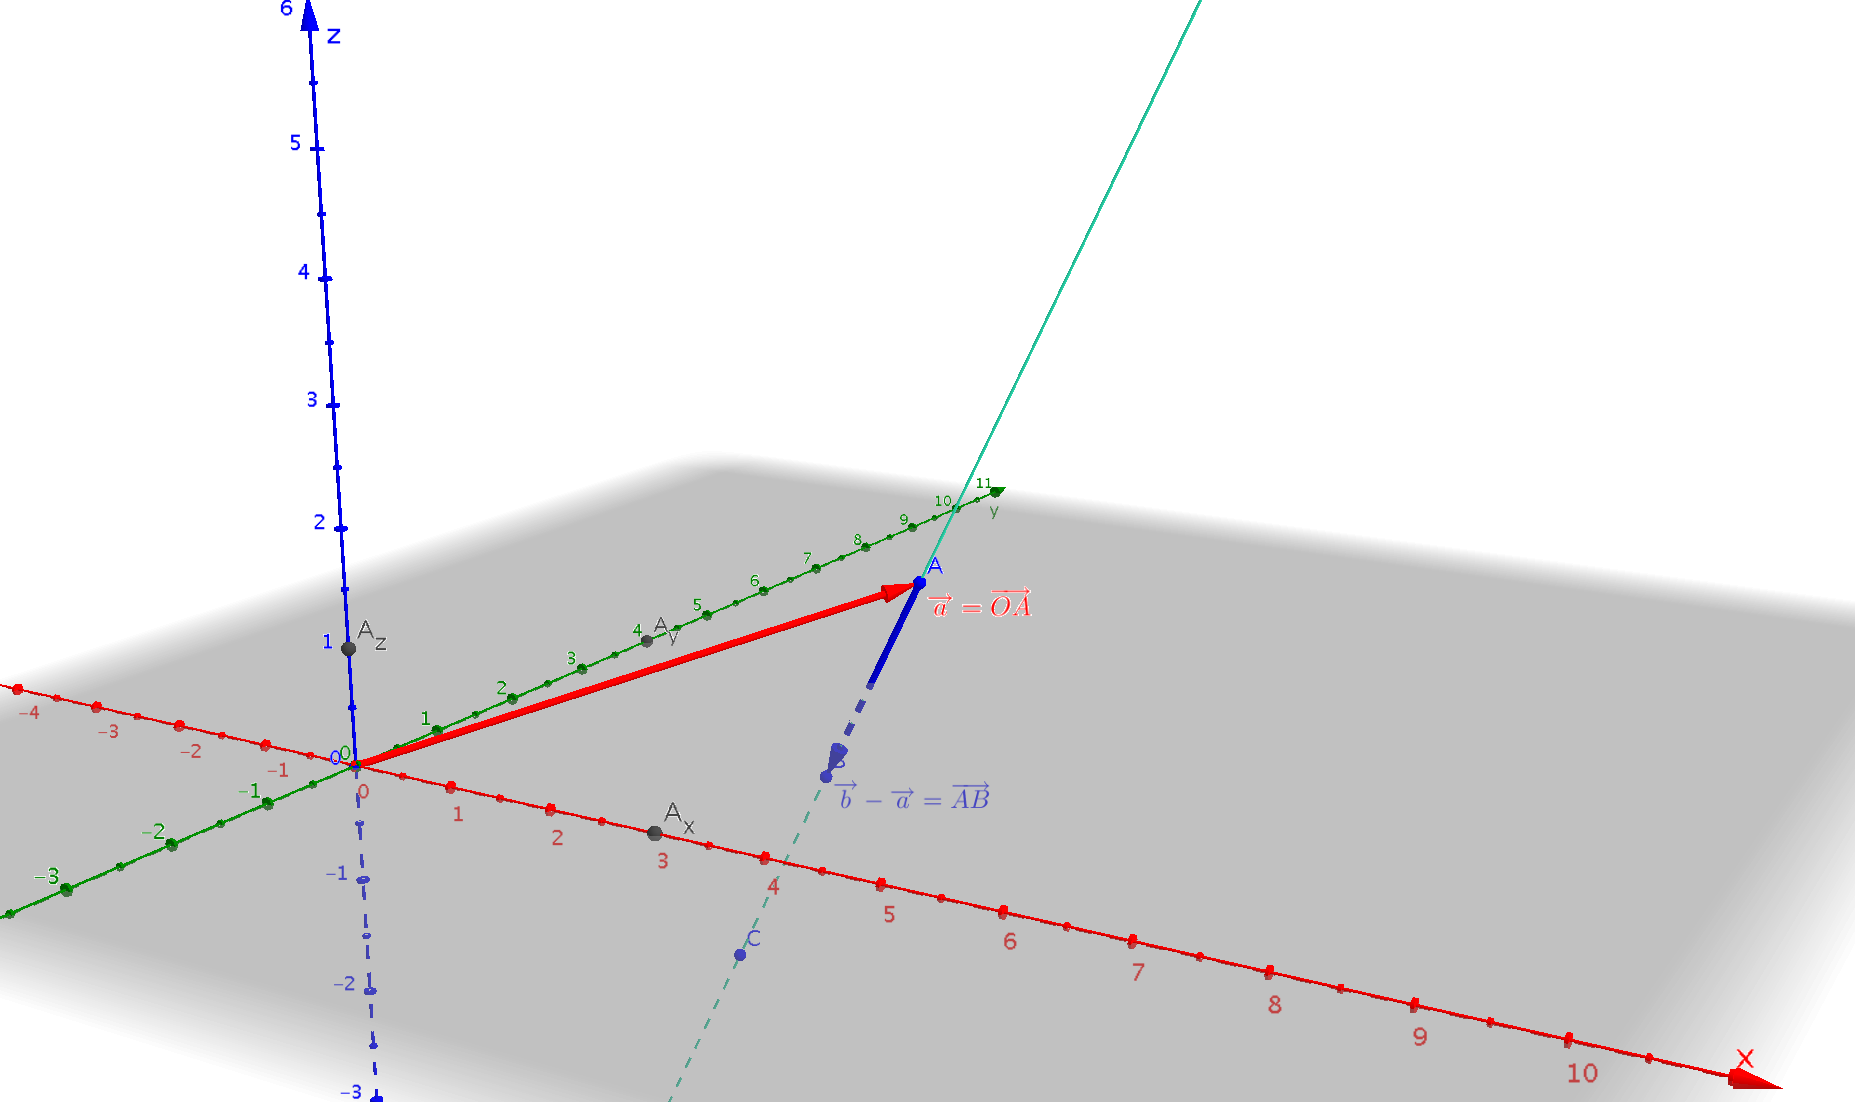
\includegraphics[width=10cm]{geradengleichung.png}
\end{frame}

\begin{frame}{Parameterdarstellung einer Geraden im $\mathbb{R}^2$}
	Eigentlich kennen Sie eine Gerade im $\mathbb{R}^2$ so:
	\[
		g = \left\{ \begin{pmatrix}
		x \\ y
		\end{pmatrix} \middle| y = m x + b \right\}
	\]
	und $b$ ist der y-Achsenabschnitt und $m$ die Steigung der Geraden.
	Das sieht dann zum Beispiel so aus:
	\definecolor{qqqqff}{rgb}{0.,0.,1.}
	\definecolor{xdxdff}{rgb}{0.49019607843137253,0.49019607843137253,1.}
	\begin{tikzpicture}[line cap=round,line join=round,>=triangle 45,x=0.6cm,y=0.6cm]
	\draw[->,color=black] (-2.713333333333333,0.) -- (12.99333333333334,0.);
	\foreach \x in {-2.,-1.,1.,2.,3.,4.,5.,6.,7.,8.,9.,10.,11.,12.}
	\draw[shift={(\x,0)},color=black] (0pt,2pt) -- (0pt,-2pt) node[below] {\footnotesize $\x$};
	\draw[->,color=black] (0.,-5.233333333333338) -- (0.,4.1);
	\foreach \y in {-5.,-4.,-3.,-2.,-1.,1.,2.,3.,4.}
	\draw[shift={(0,\y)},color=black] (2pt,0pt) -- (-2pt,0pt) node[left] {\footnotesize $\y$};
	\draw[color=black] (0pt,-10pt) node[right] {\footnotesize $0$};
	\clip(-2.713333333333333,-5.233333333333338) rectangle (12.99333333333334,4.1);
	\draw [domain=-2.713333333333333:12.99333333333334] plot(\x,{(-8.--2.*\x)/4.});
	\draw [->] (0.,-2.) -- (4.,-2.);
	\draw [->] (4.,-2.) -- (4.,0.);
	\draw (1.4066666666666687,-1.80666666666667) node[anchor=north west] {$\Delta x \, = \,4$};
	\draw (4.0466666666666695,-0.74) node[anchor=north west] {$\Delta y \, = \,2$};
	\draw (6.62,-2.24) node[anchor=north west] {$b \, = \,-2$};
	\draw (6.56666666666667,-1.36666666666667) node[anchor=north west] {$m \, = \, \frac{\Delta y}{\Delta x} \, = \,\frac{1}{2}$};
	\begin{scriptsize}
	\draw [fill=xdxdff] (0.,-2.) circle (1.5pt);
	\draw[color=xdxdff] (0.08666666666666821,-1.80666666666667) node {$A$};
	\draw [fill=qqqqff] (4.,0.) circle (1.5pt);
	\draw[color=qqqqff] (4.08666666666667,0.19333333333333036) node {$B$};
	\draw[color=black] (7.046666666666666,3.06) node {$g: y = \frac{1}{2}x - 2$};
	\end{scriptsize}
	\end{tikzpicture}
\end{frame}


\begin{frame}{Parameterdarstellung Gerade im $\mathbb{R}^2$}
	Auf dieser Geraden $y=mx+b$ liegen z.B. die Punkte
	\[
	A = \begin{pmatrix} 0 \\ b \end{pmatrix}
	\mbox{ und }
	B = \begin{pmatrix} -\frac{b}{m}\\ 0 \end{pmatrix}
	\mbox{ oder }
	D = \begin{pmatrix} 1 \\ m + b \end{pmatrix}
	\]
	\definecolor{uuuuuu}{rgb}{0.26666666666666666,0.26666666666666666,0.26666666666666666}
	\definecolor{ffxfqq}{rgb}{1.,0.4980392156862745,0.}
	\definecolor{qqqqff}{rgb}{0.,0.,1.}
	\definecolor{xdxdff}{rgb}{0.49019607843137253,0.49019607843137253,1.}
	\begin{tikzpicture}[line cap=round,line join=round,>=triangle 45,x=0.6cm,y=0.6cm]
	\draw[->,color=black] (-2.7133333333333325,0.) -- (12.99333333333334,0.);
	\foreach \x in {-2.,-1.,1.,2.,3.,4.,5.,6.,7.,8.,9.,10.,11.,12.}
	\draw[shift={(\x,0)},color=black] (0pt,2pt) -- (0pt,-2pt) node[below] {\footnotesize $\x$};
	\draw[->,color=black] (0.,-5.233333333333337) -- (0.,4.1);
	\foreach \y in {-5.,-4.,-3.,-2.,-1.,1.,2.,3.,4.}
	\draw[shift={(0,\y)},color=black] (2pt,0pt) -- (-2pt,0pt) node[left] {\footnotesize $\y$};
	\draw[color=black] (0pt,-10pt) node[right] {\footnotesize $0$};
	\clip(-2.7133333333333325,-5.233333333333337) rectangle (12.99333333333334,4.1);
	\draw [domain=-2.7133333333333325:12.99333333333334] plot(\x,{(-8.--2.*\x)/4.});
	\draw [->,line width=2.pt,color=ffxfqq] (0.,0.) -- (0.,-2.);
	\draw [->] (0.,-2.) -- (4.,-2.);
	\draw [->] (4.,-2.) -- (4.,0.);
	\draw (1.3933333333333358,-1.80666666666667) node[anchor=north west] {$\Delta x \, = \,4$};
	\draw (4.0466666666666695,-0.74) node[anchor=north west] {$\Delta y \, = \,2$};
	\draw (6.62,-2.24) node[anchor=north west] {$b \, = \,-2$};
	\draw (6.553333333333337,-1.36666666666667) node[anchor=north west] {$m \, = \frac{\Delta y}{\Delta x} \, = \,\frac{1}{2}$};
	\draw [->] (0.,0.) -- (1.,-1.5);
	\begin{scriptsize}
	\draw [fill=xdxdff] (0.,-2.) circle (1.5pt);
	\draw[color=xdxdff] (0.08666666666666858,-1.80666666666667) node {$A$};
	\draw [fill=qqqqff] (4.,0.) circle (1.5pt);
	\draw[color=qqqqff] (4.08666666666667,0.19333333333333036) node {$B$};
	\draw[color=black] (7.046666666666666,3.06) node {$g: y = \frac{1}{2}x - 2$};
	\draw [fill=uuuuuu] (1.,-1.5) circle (1.5pt);
	\draw[color=uuuuuu] (1.086666666666669,-1.3133333333333366) node {$D$};
	\end{scriptsize}
	\end{tikzpicture}
\end{frame}

\begin{frame}{Zusammenhang zwischen Geradengleichungen}
	Für eine Gerade $g$ mit der Funktionsgleichung
	\[
	g: y = m x + b \qquad x \in \mathbb{R}
	\]
	gilt also zum Beispiel:
	\[
	g = \left\{ \vv{a} = \begin{pmatrix}x \\ y\end{pmatrix} \in \mathbb{R}^2 \middle| \vv{a} = \begin{pmatrix}
	0 \\ b
	\end{pmatrix} + \lambda \begin{pmatrix}
	-\frac{b}{m} \\ -b
	\end{pmatrix}, \lambda \in \mathbb{R} \right\}
	\]
	Umgekehrt gilt für eine Gerade
	\[
	g = \left\{ \begin{pmatrix}x \\ y\end{pmatrix} \in \mathbb{R}^2 \middle| \begin{pmatrix}
	x \\ y
	\end{pmatrix} = \vv{a}  + \lambda \vv{b}, \lambda \in \mathbb{R} \right\}
	\]
	wegen $\lambda = \frac{x-a_x}{b_x}$ \footnote{also auch nur, wenn $b_x \neq 0$ ist} die Funktionsdarstellung
	\[
	g: y = a_y + \frac{b_y}{b_x} \left( x - a_x \right) = \frac{b_y}{b_x} x + \left(a_y - \frac{b_y}{b_x} a_x\right)
	\]
\end{frame}


\begin{frame}{Anwendungsbeispiel - Diagonalen im Parallelogramm}
	\begin{theorem}
		In einem Parallelogramm halbieren sich die Diagonalen.
	\end{theorem}
	\definecolor{uuuuuu}{rgb}{0.26666666666666666,0.26666666666666666,0.26666666666666666}
	\definecolor{qqqqff}{rgb}{0.,0.,1.}
	\begin{tikzpicture}[line cap=round,line join=round,>=triangle 45,x=1.0cm,y=1.0cm]
	\draw[->,color=black] (-0.31333333333333263,0.) -- (10.15777777777778,0.);
	\foreach \x in {,0.5,1.,1.5,2.,2.5,3.,3.5,4.,4.5,5.,5.5,6.,6.5,7.,7.5,8.,8.5,9.,9.5,10.}
	\draw[shift={(\x,0)},color=black] (0pt,2pt) -- (0pt,-2pt) node[below] {\footnotesize $\x$};
	\draw[->,color=black] (0.,-0.19333333333333416) -- (0.,6.028888888888882);
	\foreach \y in {,0.5,1.,1.5,2.,2.5,3.,3.5,4.,4.5,5.,5.5,6.}
	\draw[shift={(0,\y)},color=black] (2pt,0pt) -- (-2pt,0pt) node[left] {\footnotesize $\y$};
	\draw[color=black] (0pt,-10pt) node[right] {\footnotesize $0$};
	\clip(-0.31333333333333263,-0.19333333333333416) rectangle (10.15777777777778,6.028888888888882);
	\draw [->] (1.,2.) -- (6.,2.);
	\draw [->] (1.,2.) -- (2.,5.);
	\draw [->] (6.,2.) -- (7.,5.);
	\draw [->] (2.,5.) -- (7.,5.);
	\draw [->] (1.,2.) -- (7.,5.);
	\draw [->] (2.,5.) -- (6.,2.);
	\draw (2.264444444444446,3.077777777777774) node[anchor=north west] {$\vv{a}+\vv{b}$};
	\draw (2.8755555555555574,4.688888888888884) node[anchor=north west] {$\vv{a}- \vv{b}$};
	\draw [domain=-0.31333333333333263:10.15777777777778] plot(\x,{(--9.--3.*\x)/6.});
	\draw [domain=-0.31333333333333263:10.15777777777778] plot(\x,{(--26.-3.*\x)/4.});
	\begin{scriptsize}
	\draw [fill=qqqqff] (1.,2.) circle (1.5pt);
	\draw[color=qqqqff] (1.0644444444444454,2.126666666666664) node {$A$};
	\draw [fill=qqqqff] (2.,5.) circle (1.5pt);
	\draw[color=qqqqff] (2.06,5.122222222222216) node {$D$};
	\draw [fill=qqqqff] (6.,2.) circle (1.5pt);
	\draw[color=qqqqff] (6.06,2.126666666666664) node {$B$};
	\draw[color=black] (3.5177777777777797,2.108888888888886) node {$\vv{a}$};
	\draw[color=black] (1.4911111111111122,3.58444444444444) node {$\vv{b}$};
	\draw [fill=qqqqff] (7.,5.) circle (1.5pt);
	\draw[color=qqqqff] (7.0644444444444465,5.122222222222216) node {$C$};
	\draw [fill=qqqqff] (7.,5.) circle (1.5pt);
%	\draw[color=qqqqff] (7.091111111111114,5.122222222222216) node {$D'$};
	\draw [fill=uuuuuu] (4.,3.5) circle (1.5pt);
	\draw[color=uuuuuu] (4.06,3.8288888888888846) node {$S_d$};
	\end{scriptsize}
	\end{tikzpicture}
	
\end{frame}

\begin{frame}{Beweis: Diagonalen im Parallelogramm halbieren sich}
		\begin{scriptsize}

		\textbf{Denn:} Das Parallelogramm werde aufgespannt von den Vektoren $\vv{a}$ und $\vv{b}$.
		Der Schnittpunkt der Diagonalen ist der Schnittpunkt der beiden Geraden
		\[
		\vv{OA} + \vv{b} + \lambda \left(\vv{a} - \vv{b}\right) \mbox{ und } 	\vv{OA} + \mu \left(\vv{a} + \vv{b}\right)
		\]
		Der Schnittpunkt der beiden Geraden muß  beide Gleichungen erfüllen, also
		\[
		\cancel{\vv{OA}} + \vv{b} + \lambda \left(\vv{a} - \vv{b}\right) =	\cancel{\vv{OA}} + \mu \left(\vv{a} + \vv{b}\right)
		\]
		oder nach Sortierung der Terme nach $\vv{a}$ und $\vv{b}$ \[
		\left(1-\lambda-\mu\right) \vv{b} = \left(\mu - \lambda \right) \vv{a}
		\]
		Wäre nun $\mu - \lambda \neq 0$, so könnte man beide Seite durch $\mu - \lambda$ dividieren und erhielte:
		\[
		\frac{1 - \lambda - \mu}{\mu - \lambda} \vv{b} = \vv{a}
		\]
		Dann aber wären $\vv{a}$ und $\vv{b}$ parallel und könnten kein Parallelogramm aufspannen.
		
		Also ist $\mu = \lambda$ und genauso auch $1 - \mu - \lambda = 0$, also
		\[
		\lambda = \mu = \frac{1}{2}
		\]
		\end{scriptsize}
\end{frame}

\subsubsection{Ebenen}

\begin{frame}{Ebenen - Parameterdarstellung}
	Eine Ebene ist durch die Angabe dreier Punkte auf ihr eindeutig bestimmt.
	
	Sind $A$, $B$ und $C$ drei (verschiedene) Punkte und $\vv{a}$, $\vv{b}$ und $\vv{c}$ die dazugehörigen Ortsvektoren, so kann man die Menge der Punkte der Ebene $E(A,B,C)$ durch die Punkte $A$, $B$ und $C$ definieren als:
	\[
		E(A,B,C) := \left\{ \vv{y} \in \mathbb{R}^n \middle| \vv{y} = \vv{a} + \lambda \left(\vv{b} - \vv{a} \right) + \mu \left(\vv{c} - \vv{a} \right); \lambda, \mu \in \mathbb{R} \right\}
	\]
	Diese Darstellung einer Ebene heißt \textbf{Parameterdarstellung der Ebene}. Die Parameter sind hier $\lambda$ und $\mu$.
\end{frame}

\begin{frame}{Parameterdarstellung einer Ebene - Beispiel}
	
	{\footnotesize Für die Punkte $A=\begin{pmatrix}1\\2\\3\end{pmatrix}$, $B=\begin{pmatrix}3\\-1\\3\end{pmatrix}$ und $C=\begin{pmatrix}4\\-3\\0\end{pmatrix}$ ist
	\[
	E(A,B,C):= \left\{ \vv{y} \in \mathbb{R} \middle| \vv{y} = \begin{pmatrix}
	1\\2\\3
	\end{pmatrix} + \lambda \begin{pmatrix}
	2\\-3\\0
	\end{pmatrix} + \mu \begin{pmatrix}
	3\\-5\\-3
	\end{pmatrix} \right\}
	\]
	Dabei ist z.B.
	\begin{itemize}
	\item für $\lambda = 0$ und $\mu = 0$ der Punkt $A$ mit dem Ortsvektor $\begin{pmatrix}1\\2\\3\end{pmatrix}$
	\item für $\lambda = 1$ und $\mu = 0$ der Punkt $B$ mit dem Ortsvektor $\begin{pmatrix}3\\-1\\3\end{pmatrix}$
	\item für $\lambda = 0$ und $\mu = 1$ der Punkt $C$ mit dem Ortsvektor $\begin{pmatrix}4\\-3\\0\end{pmatrix}$
	\item für $\lambda = 1$ und $\mu = 1$ der Punkt $D$ mit dem Ortsvektor $\begin{pmatrix}6\\-6\\0\end{pmatrix}$
	\end{itemize}}
\end{frame}

\begin{frame}{Parameterdarstellung einer Ebene - Grafik}
	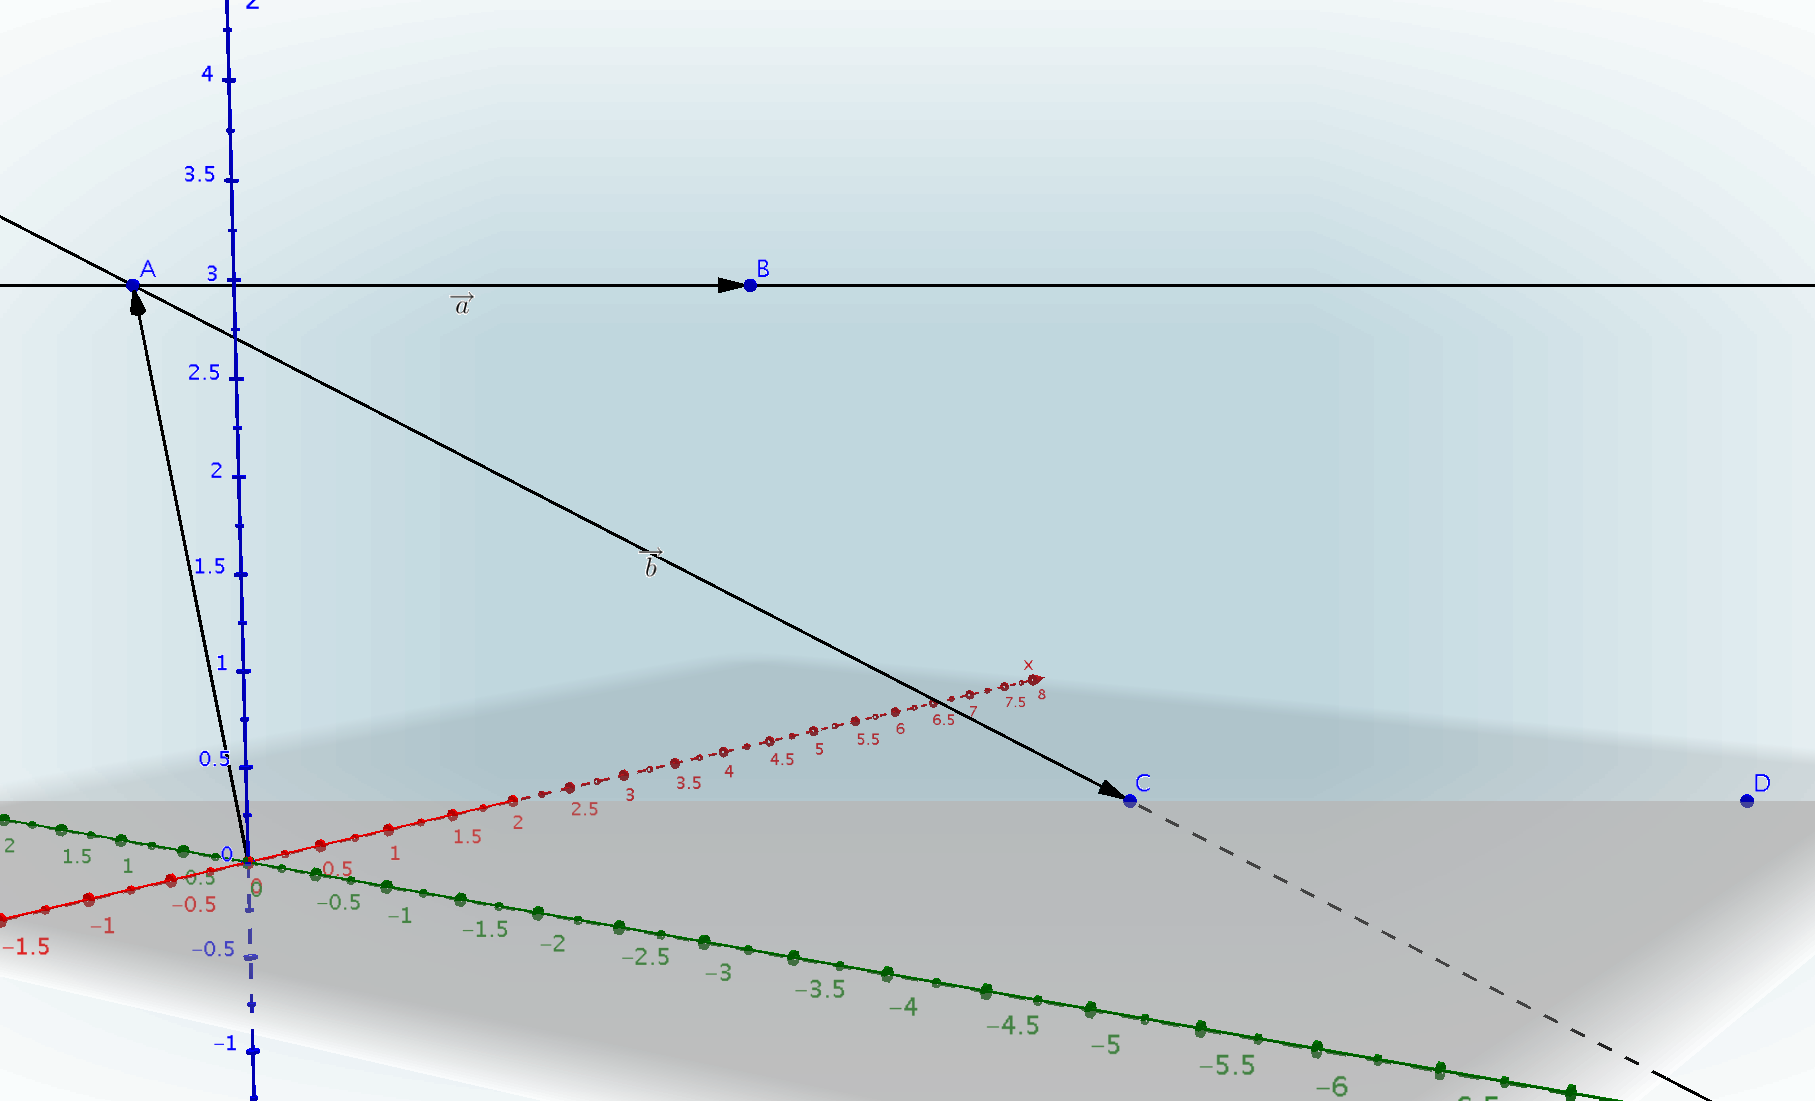
\includegraphics[width=10cm,height=8cm]{ebenengleichung.png}
\end{frame}

\begin{frame}{Normalenform einer Ebene}
	Man kann eine Ebene algebraisch auch anders darstellen.
	
	Diese Darstellung beruht auf der Idee, daß  es einen Vektor $\vv{n}$ gibt, der auf der Ebene senkrecht steht, d.h. der Vektor steht senkrecht auf allen in der Ebene liegenden Vektoren, also insbesondere auch
	\[ \vv{n} \perp \vv{u} = \vv{n} \perp (\vv{b} - \vv{a}) \qquad\mbox{und}\qquad
	\vv{n} \perp \vv{v} = \vv{n} \perp (\vv{c} - \vv{a})\]
	Es gibt aber einen speziellen Vektor, der sowohl auf $\vv{u}$ als auch auf $\vv{v}$ senkrecht steht:
	\[
		\vv{n} = \vv{u} \times \vv{v}
	\]
	Für alle Punkte der Ebene gilt damit
	\begin{framed}
		\begin{center}
		\textbf{Normalenform einer Ebene}\end{center}
	\[
	E(A,B,C) = \left\{ \vv{y} \in \mathbb{R}^3 \middle| \vv{n} \cdot \left( \vv{y} - \vv{a}\right) = 0 \right\}
	\]
	\end{framed}
\end{frame}

\begin{frame}{Umrechnung der Parameterform in Normalform}
	Um von einer Parameterdarstellung
	\[
			E = \left\{ \vv{y} \in \mathbb{R}^n \middle| \vv{y} = \vv{a} + \lambda \vv{u}  + \mu \vv{v}; \lambda, \mu \in \mathbb{R} \right\}
	\]
	in die Normalenform umzurechnen, geht man wie folgt vor:
	\begin{enumerate}
		\item Berechnung des Normalenvektors
		\[
		\vv{n} = \begin{pmatrix}
		n_1 \\ n_2 \\ n_3
		\end{pmatrix} = \vv{u} \times \vv{v}
		\]
		\item Berechnung des Skalarproduktes
		\[
		c = \vv{n} \cdot \vv{a} = n_1 a_1 + n_2 a_2 + n_3 a_3
		\]
		\item Die Normalenform ist dann
		\[
		\vv{n} \cdot \vv{y} = \vv{n} \cdot \vv{a} = 0 \Leftrightarrow n_1 y_1 + n_2 y_2 + n_3 y_3 = c
		\]
	\end{enumerate}	
\end{frame}

\begin{frame}{Umrechnung Normalform in Parameterform}
	Um von der Normalform
	\[
	E = \vv{n} \cdot \vv{y} = n_1 y_1 + n_2 y_2 + n_3 y_3 = c
	\]
	in die Parameterdarstellung umzurechnen geht man wie folgt vor:
	\begin{enumerate}
		\item Berechnung dreier Punkte der Ebene mittels der Normalform, z.B.
		\[
		A = \begin{pmatrix}
		\frac{c}{n_1} \\0 \\0
		\end{pmatrix} \qquad B = \begin{pmatrix}
		0\\ \frac{c}{n_2} \\ 0
		\end{pmatrix} \qquad C = \begin{pmatrix}
		0\\ 0 \\ \frac{c}{n_3}
		\end{pmatrix}
		\]
		\item Berechnung eines Ortsvektors und der beiden Richtungsvektoren
		\[
		\vv{a} := \vv{OA}\]
		und
		\[
		\vv{u} := \vv{b} - \vv{a} := \vv{OB} - \vv{a} \qquad \mbox{und}\qquad \vv{v} := \vv{c} - \vv{a} := \vv{OC} - \vv{a}
		\]
	\end{enumerate}
\end{frame}

\begin{frame}{Beispiel Normalform einer Ebene}
	Die Ebene aus dem vorherigen Beispiel
		\[
		E(A,B,C):= \left\{ \vv{y} \in \mathbb{R} \middle| \vv{y} = \begin{pmatrix}
		1\\2\\3
		\end{pmatrix} + \lambda \begin{pmatrix}
		2\\-3\\0
		\end{pmatrix} + \mu \begin{pmatrix}
		3\\-5\\-3
		\end{pmatrix} \right\}
		\]
	hat die Normalform	
	\begin{framed}
	\[
	9 y_1 + 6 y_2 - y_3 = 18
	\]
	\end{framed}
	{\footnotesize
	denn
	\[\vv{n} =
	\begin{pmatrix}
	2\\-3\\0
	\end{pmatrix} \times \begin{pmatrix}
	3\\-5\\-3
	\end{pmatrix} = \begin{pmatrix}
	(-3) \cdot (-3) - 0 \cdot 5 \\ 0 \cdot 3 - 2 \cdot (-3) \\ 2 \cdot (-5) - (-3) \cdot 3
	\end{pmatrix} = \begin{pmatrix}
	9 \\ 6 \\ -1
	\end{pmatrix}
	\]
	und
	\[
	\vv{n} \cdot \vv{a} = \begin{pmatrix}
	9 \\ 6 \\ -1
	\end{pmatrix} \cdot \begin{pmatrix}
	1\\2\\3
	\end{pmatrix} = 9\cdot 1 + 6 \cdot 2 + (-1)\cdot 3= 9 + 12 -3 = 18
	\] }
\end{frame}

\begin{frame}{Abstand Punkt-Ebene}
	Man kann mit Hilfe der Normalform einer Ebene den Abstand eines beliebigen Punktes zu dieser Ebene berechnen:
	\begin{framed}
	\begin{center}
		Abstandsformel
	\end{center}
	Der Abstand $d(P,E)$ eines Punktes $P$ mit dem Ortsvektor $\vv{p}$ zur Ebene $E : \vv{n} \cdot \left( \vv{y}  - \vv{a} \right) = 0$ ist
	\[
	d(P,E) = \frac{\vv{n} \cdot \left( \vv{p} - \vv{a} \right)}{\| \vv{n} \|} = \frac{\vv{n} \cdot \vv{p}}{\| \vv{n} \|} - \frac{\vv{n} \cdot \vv{a}}{\| \vv{n} \|}
	\]
	\end{framed}
	Man muß  also die Normalform nehmen und noch durch die Länge des Normalenvektors teilen.
\end{frame}

\subsection{Lineare Gleichungssysteme und Matrizen}
\subsubsection{Lineare Gleichungssysteme}

\begin{frame}{Lineare Algebra - Systeme linearer Funktionen und Gleichungen}

\begin{definition}
	
	Ein System von m linearen Gleichungen mit n Unbekannten der Form
\begin{align*}
a_{11} x_{1} + a_{12} x_{2} + a_{13} x_{3} + \ldots + a_{1n} x_{n}  & =   b_{1} \\
a_{21} x_{1} + a_{22} x_{2} + a_{23} x_{3} + \ldots + a_{2n} x_{n}  & =   b_{2} \\
a_{31} x_{1} + a_{32} x_{2} + a_{33} x_{3} + \ldots + a_{3n} x_{n}  & =   b_{3} \\
\vdots \qquad &  \\
a_{m1} x_{1} + a_{m2} x_{2} + a_{m3} x_{3} + \ldots + a_{mn} x_{n}  & =   b_{m}
\end{align*}
heißt \textbf{lineares Gleichungssystem}.
\end{definition}
\begin{bemerkung}
	Hierbei sind $a_{11}$, $a_{12}, \ldots , a_{mn}$ und $b_1 , \ldots , b_m$ vorgegebene reelle Zahlen, auch \textbf{Koeffizienten} genannt. Gesucht ist die Menge der $x_1$, $x_2, \ldots , x_n$ (\textbf{Lösung des Gleichungssystems}), die das Gleichungssystem erfüllen.
\end{bemerkung}
\end{frame}

\begin{frame}{Beispiele linearer Gleichungssysteme}
	\begin{example}
		Das lineare Gleichungssystem
		\begin{align*}
		a_{11} x + a_{12} y & = b_1 \\
		a_{21} x + a_{22} y & = b_2
		\end{align*}
		besteht geometrisch aus zwei Geradengleichungen im $\mathbb{R}^{2}_{(x,y)}$. Die Lösungsmenge dieses Gleichungssystems besteht aus all den Punkten, die auf beiden Geraden liegen, also gilt entweder
		\begin{itemize}
			\item die Lösungsmenge besteht genau aus dem Schnittpunkt der beiden Geraden oder
			\item die Lösungsmenge besteht aus allen Punkten der Geraden, weil beide Gleichungen vielleicht dieselbe Gerade beschreiben oder
			\item die Lösungsmenge ist leer, weil die Geraden parallel sind und es daher keine gemeinsamen Punkte gibt.
		\end{itemize}
			
	\end{example}
\end{frame}

\begin{frame}{Beispiele linearer Gleichungssysteme - Genau eine Lösung}
	\begin{example}
		Das lineare Gleichungssystem
		\begin{align*}
		x + 2 y & = 1 \\
		3 x + y & = 2
		\end{align*}
		kann man lösen durch das \textbf{Einsetzungsverfahren}:
		Die erste Gleichung nach $x$ auflösen ergibt
		\[x = 1 - 2 y\]
		und dies eingesetzt in die zweite Gleichung
		\[
		3 (1 - 2y) +y = 2
\Leftrightarrow
		3 - 5 y = 2 \Leftrightarrow y = \frac{1}{5}
		\]
		und damit
		\[
		x = 1 - 2y = \frac{5}{5} - 2\frac{1}{5} = \frac{3}{5}
		\]
	\end{example}
\end{frame}
\begin{frame}{Beispiele linearer Gleichungssysteme - Unendlich viele Lösungen}
	\begin{example}
		Das lineare Gleichungssystem
				\begin{align*}
				x + 2 y & = 1 \\
				3 x +  6 y & = 3
				\end{align*}
		führt per Einsetzungsverfahren auf die Gleichung
		\[
		3  + 0 y= 3
		\]
		was unabhängig davon gilt, was für $y$ eingesetzt wird, diese Gleichung gilt also für jeden Wert von $y$.
		Daher ist die gesamte Gerade
		\[
		x = 1 - 2 y \qquad \forall y \in \mathbb{R}
		\]
		Lösungsmenge dieses linearen Gleichungssystems, es gibt also unendlich viele Lösungen (zu jedem y jeweils eine).
	\end{example}
\end{frame}

\begin{frame}{Beispiele linearer Gleichungssysteme - Keine Lösung}
	\begin{example}
		Das lineare Gleichungssystem
		\begin{align*}
		x + 2 y & = 1 \\
		3 x +  6 y & = 2
		\end{align*}
		führt per Einsetzungsverfahren auf die Gleichung
		\[
		3  + 0 y= 2
		\]
		die, unabhängig davon, was für $y$ eingesetzt wird, nicht erfüllt werden kann.
		
		Die Lösungsmenge dieses Gleichungssystems ist daher leer; die Geraden sind parallel und schneiden sich nicht.
	\end{example}
\end{frame}

\begin{frame}{Beispiele linearer Gleichungssysteme}

	\begin{example}
	Ein lineares Gleichungssystem mit nur \textbf{einer} Gleichung und n Unbekannten hat die Form
	\[
		a_1 x_1 + a_2 x_2 + \ldots + a_n x_n = b_1
	\]
	Das ist aber die Normalenform einer Ebene im $\mathbb{R}^n$ und daher ist die Lösungsmenge dieses Gleichungssystems eine (Hyper-)Ebene im $\mathbb{R}^n$.		
	\end{example}
\end{frame}

\begin{frame}{Beispiele linearer Gleichungssysteme - Mehr Gleichungen als Unbekannte}
	\begin{example}
	Das lineare Gleichungssystem
	\begin{align*}
	x - 2 y & = -4 \\
	-x + 3 y & = 5 \\
	x - y & = -3 \\
	2 x - 3 y & = -7 \\
	x + y & = -1
	\end{align*}		
	ist ein Gleichungssystem mit zwei Unbekannten und 5 Gleichungen. Es hat die Lösung $x = -2$ und $y = 1$.
	\end{example}

\end{frame}

\begin{frame}{Beispiele linearer Gleichungssysteme - Mehr Unbekannte als Gleichungen}
	\begin{example}
		Das lineare Gleichungssystem
		\begin{align*}
		x_1 - x_2 + 3 x_3 -2 x_4 + x_5 & = 1 \\
		2 x_1 -2 x_2 + 6x_3 -4 x_4 +2x_5 & = 1
		\end{align*}
		hat keine Lösung, denn die linke Seite der zweiten Gleichung ist gerade das doppelte der erste, was für die rechte Seite nicht gilt. Das heißt jede Lösung der ersten Gleichung würde die zweite nicht erfüllen können.
	\end{example}
\end{frame}

\begin{frame}{Lineare Gleichungssysteme}
	\begin{definition}
	Das lineare Gleichungssystem
	\begin{align*}
	a_{11} x_{1} + a_{12} x_{2} + a_{13} x_{3} + \ldots + a_{1n} x_{n}  & =   0 \\
	a_{21} x_{1} + a_{22} x_{2} + a_{23} x_{3} + \ldots + a_{2n} x_{n}  & =   0 \\
	a_{31} x_{1} + a_{32} x_{2} + a_{33} x_{3} + \ldots + a_{3n} x_{n}  & =   0 \\
	\vdots \qquad &  \\
	a_{m1} x_{1} + a_{m2} x_{2} + a_{m3} x_{3} + \ldots + a_{mn} x_{n}  & =   0
	\end{align*}
	heißt \textbf{homogenes} lineares Gleichungssystem.
	\end{definition}
	\begin{bemerkung}
		Ein lineares Gleichungssystem ist also genau dann homogen, wenn $b_i = 0$ für alle $i=1, 2, \ldots m$ gilt.
		Sobald auch nur für ein einziges $b_i \neq 0$ gilt, ist das Gleichungssystem nicht homogen und wird \textbf{inhomogen} genannt.
	\end{bemerkung}
\end{frame}

\begin{frame}{Lösbarkeit linearer Gleichungssysteme}
	\begin{bemerkung}
		Für ein \textbf{homogenes}, lineares Gleichungssystem mit $b_1 = b_2 = \ldots b_m = 0$ gilt:
		\begin{itemize}
			\item Entweder besitzt das System genau eine Lösung $x_1 = x_2 = \ldots x_n = 0$.
			\item Das System besitzt unendlich viele Lösungen (und eine davon ist $x_1 = x_2 = \ldots x_n = 0$).
		\end{itemize}
	\end{bemerkung}
	\begin{bemerkung}
		Für ein \textbf{inhomogenes}, lineares Gleichungssystem mit $b_i \neq 0$ für mindestens ein $i=1, \ldots m$ gilt einer von drei möglichen Fällen:
		\begin{itemize}
			\item Das Gleichungssystem besitzt keine Lösung, weil es widersprüchlich ist.
			\item Das System besitzt genau eine Lösung.
			\item Das System besitzt unendlich viele Lösungen.
		\end{itemize}
	\end{bemerkung}
\end{frame}

\begin{frame}{Lösungsmethoden für lineare Gleichungssysteme}
	Für lineare Gleichungssysteme gibt es verschiedene Lösungsverfahren:
	\begin{itemize}
		\item \textbf{Substitutionsverfahren/Einsetzungsverfahren}
		
		Bei diesem Verfahren wird die Anzahl der Gleichungen sukzessive durch Auflösen, Einsetzen und dadurch die Reduktion von Variablen verringert, bis die Lösung einer Variablen übrig bleibt. Die Lösung der anderen Variablen erfolgt dann durch sukzessives Zurück-Einsetzen der gefundenen Lösungen.
		\item \textbf{Additionsverfahren}
		
		Bei diesem Verfahren wird die Anzahl der Gleichungen sukzessive durch Addition von Gleichungen verringert, bis die Lösung einer Variablen übrig bleibt.
		
		\item \textbf{Cramersche Regel}
		
		Bei diesem Verfahren werden \textbf{Determinanten} zur Lösungsbestimmung benutzt.
		
		\item \textbf{Gauß -(Jordan-)Verfahren}
		
		Beim Gauß -(Jordan-)Verfahren wird systematisch das Additionsverfahren benutzt, um die Lösung eines linearen Gleichungssystems zu finden.
	\end{itemize}
	
\end{frame}

\begin{frame}{Lineare Gleichungssysteme in Matrizenschreibweise}
	\begin{bemerkung}
	Man kann lineare Gleichungssysteme schöner und einfacher schreiben. Für das lineare Gleichungssystem
	\begin{align*}
	a_{11} x_{1} + a_{12} x_{2} + a_{13} x_{3} + \ldots + a_{1n} x_{n}  & =   b_{1} \\
	a_{21} x_{1} + a_{22} x_{2} + a_{23} x_{3} + \ldots + a_{2n} x_{n}  & =   b_{2} \\
	a_{31} x_{1} + a_{32} x_{2} + a_{33} x_{3} + \ldots + a_{3n} x_{n}  & =   b_{3} \\
	\vdots \qquad &  \\
	a_{m1} x_{1} + a_{m2} x_{2} + a_{m3} x_{3} + \ldots + a_{mn} x_{n}  & =   b_{m}
	\end{align*}
	steckt ja alles \emph{Wichtige} in den Koeffizienten $a_{ij}$ und $b_i$.
\end{bemerkung}
\end{frame}

\begin{frame}{Lineare Gleichungssysteme in Matrizenschreibweise}
	\begin{definition}
		Das Zahlenschema
		\[
		A = \begin{pmatrix}
		a_{11} & a_{12} & a_{13} & \cdots & a_{1n} \\
		a_{21} & a_{22} & a_{23} & \cdots & a_{2n} \\
		a_{31} & a_{32} & a_{33} & \cdots & a_{3n} \\
		\vdots & \vdots & \vdots  & \ddots & \vdots \\
		a_{m1} & a_{m2} & a_{m3} & \cdots & a_{mn}
		\end{pmatrix}
		\]
		heißt $m \times n$-Matrix. Es hat $m$ Zeilen und $n$ Spalten. Das Element in der $i$-ten Zeile und in der $j$-ten Spalte ist also $a_{ij}$.
		
		Sind die Elemente $a_{ij}=0$ für alle $i,j$, so heißt die Matrix \textbf{Nullmatrix}.
		
		Die $n \times n$-Matrix $I_n$, in der alle Diagonalelemente $a_{ii}=1$ für alle i und alle anderen $a_{ij}=0$ sind, heißt \textbf{Einheitsmatrix}.
		$i$ heißt auch \textbf{Zeilenindex}, $j$ heißt \textbf{Spaltenindex}. $m$ ist die Anzahl der Zeilen, $n$ ist die Anzahl der Spalten.
	\end{definition}
\end{frame}

\begin{frame}{Beispiele für Matrizen}
		Der Vektor
		\[
		\begin{pmatrix}
		x_1 \\ x_2 \\ x_3 \\ \vdots \\ x_n
		\end{pmatrix}
		\]
		kann auch als $n \times 1$-Matrix aufgefaßt werden.
		
		Die Nullmatrix und die Einheitsmatrix sind
		\[
		\pmb{0} = \begin{pmatrix}
		0 & 0 & 0 & \cdots & 0 \\
		0 & 0 & 0 & \cdots & 0 \\
		0 & 0 & 0 & \cdots & 0 \\
		\vdots & \vdots &  \vdots & \ddots  & \vdots \\
		0 & 0 & 0 & \cdots & 0
		\end{pmatrix} \qquad \pmb{I_n} = \begin{pmatrix}
		1 & 0 & 0 & \cdots & 0 \\
		0 & 1 & 0 & \cdots & 0 \\
		0 & 0 & 1 & \cdots & 0 \\
		\vdots & \vdots &  \vdots & \ddots & \vdots \\
		0 & 0 & 0 & \cdots & 1
		\end{pmatrix}
		\]
\end{frame}

\begin{frame}{Beispiele für Matrizen}
	Es gibt auch $1 \times n$-Matrizen wie z. B.
			\[
			\begin{pmatrix}
			a_1 & a_2 & a_3 & \cdots & a_n
			\end{pmatrix}
			\]die genau aus einer Zeile bestehen.
			
			Matrizen, die genau so viele Zeilen wie Spalten haben, heiß en \textbf{quadratische Matrizen}. Z. B. ist die Matrix
			\[	
	\begin{pmatrix}
		a_{11} & a_{12} & a_{13} & \cdots & a_{1n} \\
		a_{21} & a_{22} & a_{23} & \cdots & a_{2n} \\
		a_{31} & a_{32} & a_{33} & \cdots & a_{3n} \\
		\vdots & \vdots & \vdots  & \ddots & \vdots \\
		a_{n1} & a_{n2} & a_{n3} & \cdots & a_{nn}
	\end{pmatrix}
	\]
	quadratisch.
\end{frame}

\begin{frame}{Rechenregeln für Matrizen}
	\footnotesize{
	\begin{definition}
		Vertauscht man bei einer $m \times n$-Matrix
				\[
				\pmb{A} = \begin{pmatrix}
				a_{11} & a_{12}  & \cdots & a_{1n} \\
				a_{21} & a_{22}  & \cdots & a_{2n} \\
				\vdots & \vdots   & \ddots & \vdots \\
				a_{m1} & a_{m2}  & \cdots & a_{mn}
				\end{pmatrix}
				\]
		die Zeilen und Spalten, so erhält man eine $n \times m$- Matrix, die \textbf{transponierte Matrix}
				\[
				\pmb{A^{T}} = \begin{pmatrix}
				a_{11} & a_{21}  & \cdots & a_{m1} \\
				a_{12} & a_{22}  & \cdots & a_{m2} \\
				\vdots & \vdots   & \ddots & \vdots \\
				a_{1n} & a_{2n}  & \cdots & a_{mn}
				\end{pmatrix}
				\]
		Für die Koeffizienten der transponierten Matrix $\pmb{A^{T}}$, die man mit $a^{T}_{ij}$ bezeichnen kann, gilt also:
		\[
			a^{T}_{ij} := a_{ji} \qquad \forall i=1, \ldots, n; j=1, \ldots m
		\]
				
	\end{definition}
}
\end{frame}

\begin{frame}{Beispiele - Transponierte Matrix}
		\[
		\pmb{A} = \begin{pmatrix}
		1 & 3  \\
		4 & 2 \\
		0 & -8
		\end{pmatrix}
		 \qquad 		\pmb{A^{T}} = \begin{pmatrix}
			1 & 4 & 0 \\
			3 & 2 & -8
		\end{pmatrix}
		\]
		Für quadratische Matrizen bedeutet das Transponieren nichts anderes als das Spiegeln der Koeffizienten an der Diagonalen:
		\[
				\pmb{B} = \begin{pmatrix}
				1 & 1 & 1  \\
				0 & -2 & 5\\
				7 & 6 & 0
				\end{pmatrix}
				\qquad 	\pmb{B^{T}} = \begin{pmatrix}
				1 & 0 & 7 \\
				1 & -2 & 6 \\
				1 & 5 & 0
				\end{pmatrix}		
		\]
					
\end{frame}

\begin{frame}{Rechenregeln für Matrizen}
	\begin{bemerkung}
		Zwei Matrizen $\pmb{A}$ und $\pmb{B}$ sind genau dann gleich, wenn sie
		\begin{itemize}
			\item vom gleichen Typ $(m \times n)$ sind und
			\item $a_{ij} = b_{ij}$ für alle $i= 1, 2, \ldots m$ und alle $j= 1, 2, \ldots n$.
		\end{itemize}
		Das heißt, die Matrizen haben den gleichen Typ und stimmen in allen entsprechenden Elementen überein.
\end{bemerkung}
\begin{bemerkung}
	
Zwei Matrizen $\pmb{A}$ und $\pmb{B}$ werden addiert, indem man die entsprechenden Komponenten addiert:
\scriptsize{
\[
\begin{pmatrix}
a_{11} & \cdots & a_{1n} \\
a_{21} & \cdots & a_{2n} \\
\vdots & \ddots & \vdots \\
a_{m1} & \cdots & a_{mn}
\end{pmatrix} + \begin{pmatrix}
b_{11} & \cdots & b_{1n} \\
b_{21} & \cdots & b_{2n} \\
\vdots & \ddots & \vdots \\
b_{m1} & \cdots & b_{mn}
\end{pmatrix} = \begin{pmatrix}
a_{11} + b_{11} & \cdots & a_{1n} + b_{1n} \\
a_{21} + b_{21} & \cdots & a_{2n} +b_{2n}\\
\vdots & \ddots & \vdots \\
a_{m1} + b_{m1} & \cdots & a_{mn} + b_{mn}
\end{pmatrix}
\]
}{\normalsize
Insbesondere müssen die Matrizen denselben Typ haben!}
\end{bemerkung}
\end{frame}

\begin{frame}{Multiplikation mit einem Skalar}
	\begin{bemerkung}
		Eine Matrix $\pmb{A}$ wird mit einem Skalar $\lambda$ multipliziert, indem man jedes Matrixelement $a_{ij}$ mit dem Skalar multipliziert:
		\[
		\lambda \pmb{A} := \lambda \begin{pmatrix}
			a_{11} & a_{12} & \cdots & a_{1n} \\
			a_{21} & a_{22} & \cdots & a_{2n} \\
			\vdots & \vdots & \ddots & \vdots \\
 			a_{m1} & a_{m2} & \cdots & a_{mn} \\
		\end{pmatrix} := \begin{pmatrix}
		\lambda a_{11} & \lambda a_{12} & \cdots & \lambda a_{1n} \\
		\lambda a_{21} & \lambda a_{22} & \cdots & \lambda a_{2n} \\
		\vdots & \vdots & \ddots & \vdots \\
		\lambda a_{m1} & \lambda a_{m2} & \cdots & \lambda a_{mn} \\
		\end{pmatrix}
		\]
	\end{bemerkung}
\end{frame}

\begin{frame}{Rechnen mit Matrizen}
	\begin{definition}
		Für eine $k \times m$-Matrix $\pmb{A}$ und eine $m \times n$-Matrix $\pmb{B}$
		\[
		\pmb{A} = \begin{pmatrix}
		a_{11} & a_{12}  & \cdots & a_{1m} \\
		a_{21} & a_{22}  & \cdots & a_{2m} \\
		\vdots & \vdots   & \ddots & \vdots \\
		a_{k1} & a_{k2}  & \cdots & a_{km}
		\end{pmatrix} \qquad \pmb{B} = \begin{pmatrix}
		b_{11} & b_{12}  & \cdots & b_{1n} \\
		b_{21} & b_{22}  & \cdots & b_{2n} \\
		\vdots & \vdots   & \ddots & \vdots \\
		b_{m1} & b_{m2}  & \cdots & b_{mn}
		\end{pmatrix}
		\] definiert man das \textbf{Matrixprodukt} als die $k \times n$-Matrix $\pmb{C}$
		\[
		\pmb{C} = \pmb{A} \cdot \pmb{B} := \begin{pmatrix}
		c_{11} & c_{12} & c_{13} & \cdots & c_{1n} \\
		c_{21} & c_{22} & c_{23} & \cdots & c_{2n} \\
		\vdots & \vdots & \vdots  & \ddots & \vdots \\
		c_{k1} & c_{m2} & c_{k3} & \cdots & c_{kn}
		\end{pmatrix}
		\]
		für die gilt:
		
		\fbox{
			$c_{ij} = \sum_{l=1}^{m} a_{il} b_{lj} = a_{i1} b_{1j} + a_{i2} b_{2j} + a_{i3} b_{3j} + \cdots + a_{im} b_{mj}$}.
	\end{definition}
\end{frame}

\begin{frame}{Hinweise zum Matrizenprodukt}
	\begin{bemerkung}
	Das Element $c_{ij}$ der Produktmatrix entsteht also, indem man die $i$-te Zeile von $\pmb{A}$ mit der $j$-ten Spalte von $\pmb{B}$ komponentenweise multipliziert:

\[
c_{ij} = \left( \pmb{A} \cdot \pmb{B} \right)_{ij} := \sum_{l=1}^{m} a_{il} b_{lj}
\]	
	Natürlich muß  dafür $\pmb{A}$ genau so viele Spalten(!) haben wie $\pmb{B}$ Zeilen(!) hat, nämlich $m$.
	
	Die Produktmatrix hat dieselbe Anzahl an Zeilen wie $\pmb{A}$ und dieselbe Anzahl an Spalten wie $\pmb{B}$, weil es für jede Zeile von $\pmb{A}$ (Index $i$) und jede Spalte von $\pmb{B}$ (Index $j$) einen entsprechenden Eintrag $c_{ij}$ gibt.	
	
	\fbox{\scriptsize{Das Produkt einer $k \times m$-Matrix mit einer $m \times n$- Matrix ergibt also eine $k \times n$-Matrix.}}
	\end{bemerkung}
\end{frame}

\begin{frame}{Schema von Falk (nach Sigurd Falk)}
	Die Durchf"uhrung der Matrizenmultiplikation kann mit Hilfe des
	\textbf{Schemas von Falk} erfolgen:
	\begin{equation*}
	\begin{array}{@{}rl}
	\pmb{B} \ = \
	\left(
	\begin{array}{c} b_{11} \\ \vdots \\ b_{p1}
	\end{array}
	\begin{array}{c} \cdots \\   \\ \cdots \end{array}
	\fbox{$\begin{array}{c} b_{1k} \\ \vdots \\ b_{pk}
		\end{array}$}
	\begin{array}{c} \cdots \\   \\ \cdots \end{array}
	\begin{array}{c} b_{1n} \\ \vdots \\ b_{pn}
	\end{array}
	\right) \, &
	\\
	\pmb{A} \ = \
	\left(
	\begin{array}{c}
	a_{11} \quad \cdots \quad a_{1p} \\
	\ \vdots \hfill \vdots \quad  \\
	\fbox{$a_{i1} \quad \cdots \quad a_{ip}$} \\
	\ \vdots \hfill \vdots \quad \\
	a_{m1} \quad \cdots \quad a_{mp}
	\end{array} \right) \
	\left(
	\begin{array}{c} c_{11} \\ \vdots \\ c_{i1} \\
	\vdots \\ c_{m1}          \end{array}
	\begin{array}{c} \cdots \\   \\ \cdots \\ \\ \cdots \end{array}
	\begin{array}{c} c_{1k} \\ \vdots \\ \fbox{$c_{ik}$} \\
	\vdots \\ c_{mk}
	\end{array}
	\begin{array}{c} \cdots \\   \\ \cdots \\ \\ \cdots \end{array}
	\begin{array}{c} c_{1n} \\ \vdots \\ c_{in} \\
	\vdots \\ c_{mn}          \end{array}
	\right) &  = \ \pmb{C}
	\end{array}
	\end{equation*}
	
	\textbf{Beispiel:} $\quad \!
	\pmb{B} = \left( \begin{array}{rrr} 4 & \ 7 & \ 6 \\
	-2 & 3 & 1 \end{array} \right)$
	
	$\pmb{A} = \left( \begin{array}{rr}  0 & 3 \\
	4 & 2 \\ 1 & 0 \end{array} \right) \
	\left( \begin{array}{rrr} -6 & 9 & 3 \\
	12 & 34 & 26 \\
	4 & 7 & 6 \end{array} \right)
	= \pmb{C}$
	
\end{frame}

\begin{frame}{Rechenregeln für Matrizenprodukte}
	\begin{bemerkung}
		Für das Matrizenprodukt gelten folgende Regeln (wenn man die Produkte überhaupt bilden kann):
		\begin{align*}
		\left( \pmb{A} \pmb{B}\right)\pmb{C} & = \pmb{A} \left(\pmb{B} \pmb{C}\right) \qquad &\mbox{Assoziativgesetz} \\
		\pmb{A} \left( \pmb{B} + \pmb{C} \right) & = \pmb{A} \pmb{B} + \pmb{A} \pmb{C} \qquad &\mbox{Distributivgesetz links} \\
		\left( \pmb{B} + \pmb{C} \right) \pmb{A} & =  \pmb{B}\pmb{A} + \pmb{C} \pmb{A} \qquad &\mbox{Distributivgesetz rechts} \\
		\end{align*}
		Es gilt aber nicht(!) das Kommutativgesetz:
		\[
		\pmb{A} \pmb{B} \neq \pmb{B} \pmb{A}
		\]
	\end{bemerkung}
\end{frame}

\begin{frame}{Lineare Gleichungssysteme in Matrizenschreibweise}
\begin{bemerkung}
	Ein lineares Gleichungssystem kann man in Matrizenschreibweise auch so schreiben:
	\[
	\begin{pmatrix}
	a_{11} & a_{12}  & \cdots & a_{1n} \\
	a_{21} & a_{22}  & \cdots & a_{2n} \\
	\vdots & \vdots   & \ddots & \vdots \\
	a_{m1} & a_{m2}  & \cdots & a_{mn}
	\end{pmatrix} \cdot \begin{pmatrix}
	x_1 \\ x_2 \\ \vdots \\ x_n
	\end{pmatrix} = \begin{pmatrix}
	b_1 \\ b_2 \\ \vdots \\ b_m
	\end{pmatrix}
	\]
\end{bemerkung}
\end{frame}

\begin{frame}{Lösungsverfahren für lineare Gleichungssysteme}
	\begin{bemerkung}
		Eines der wichtigsten Lösungsverfahren für lineare Gleichungssysteme ist das \textbf{Gauß -Jordan-Verfahren}:
		
		Die folgenden Umformungen ändern die Lösungsmenge eines linearen Gleichungssystems nicht und können daher auf ein gegebenes lineares Gleichungssystem beliebig oft angewendet werden. Diese Umformungen heißen \textbf{elementare} oder auch \textbf{zulässige Umformungen eines linearen Gleichungssystems}:
		\begin{itemize}
			\item Vertauschen zweier Zeilen(!).
			\item Multiplikation einer Zeile(!) mit einer von 0 verschiedenen Zahl.
			\item Addition einer Zeile(!) auf eine andere Zeile(!).
		\end{itemize}
		Wenn man diese Umformungen geschickt anwendet, findet man die Lösungsmenge jedes linearen Gleichungssystems, auch wenn diese leer ist.
	\end{bemerkung}
\end{frame}

\begin{frame}{Anwendungsbeispiel - Matrizenmultiplikation}
Drei Anbieter eines Produktes haben in einer bestimmten Periode (1) Marktanteile von 40\%, 20\% bzw. 40\%. Die Marktentwicklung wird durch die folgende Abbildung wiedergegeben.

\textbf{Wie sind die Marktanteile in der Folgeperiode (2)?}
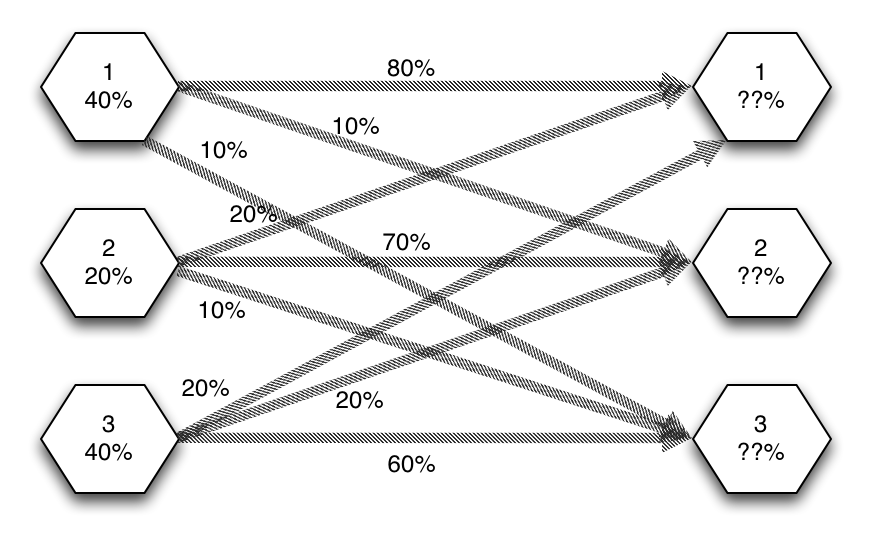
\includegraphics[width=10cm]{marktanteile.png}
\end{frame}

\begin{frame}{Anwendungsbeispiel - Matrizenmultiplikation}
	Darstellung der Marktanteile in den beiden Perioden:
	\[
	\pmb{M^{1}} = \begin{pmatrix}m^{1}_{1}  \\ m^{1}_{2} \\ m ^{1}_{3}\end{pmatrix} = \begin{pmatrix}40 \% \\ 20 \% \\ 40 \%\end{pmatrix} \qquad \pmb{M^{2}} = \begin{pmatrix}m^{2}_{1}  \\ m^{2}_{2} \\ m^{2}_{3}\end{pmatrix}
	\]
	
	Darstellung der Übergänge der Marktanteile durch eine Übergangsmatrix:
	\[
	\pmb{K^{12}} = \begin{pmatrix}
		k^{12}_{11} & k^{12}_{12} & k^{12}_{13} \\
		k^{12}_{21} & k^{12}_{22} & k^{12}_{23} \\
		k^{12}_{31} & k^{12}_{32} & k^{12}_{33} \\
	\end{pmatrix}
	\]
	
	\textbf{$k^{12}_{ij}$ gibt den Anteil des Übergangs von Produzent $j$ auf Produzent $i$ an beim Wechsel von Periode 1 auf Periode 2!}
	
	Die Marktanteile $\pmb{M_{2}}$ in Periode 2 sind dann:
	\[
		\pmb{M^{2}} = \pmb{K^{12}} \pmb{M^{1}}
	\]
\end{frame}

\begin{frame}{Anwendungsbeispiel - Matrizenmultiplikation}
	\[
	\pmb{M^{2}} = \pmb{K^{12}} \pmb{M^{1}} = \begin{pmatrix}
		0,8 & 0,2 & 0,2 \\
		0,1 & 0,7 & 0,2 \\
		0,1 & 0,1 & 0,6
	\end{pmatrix} \begin{pmatrix}
		40\% \\ 20 \% \\ 40 \%
	\end{pmatrix} = \begin{pmatrix}
		44\% \\ 26 \% \\ 30 \%
	\end{pmatrix}
	\]
	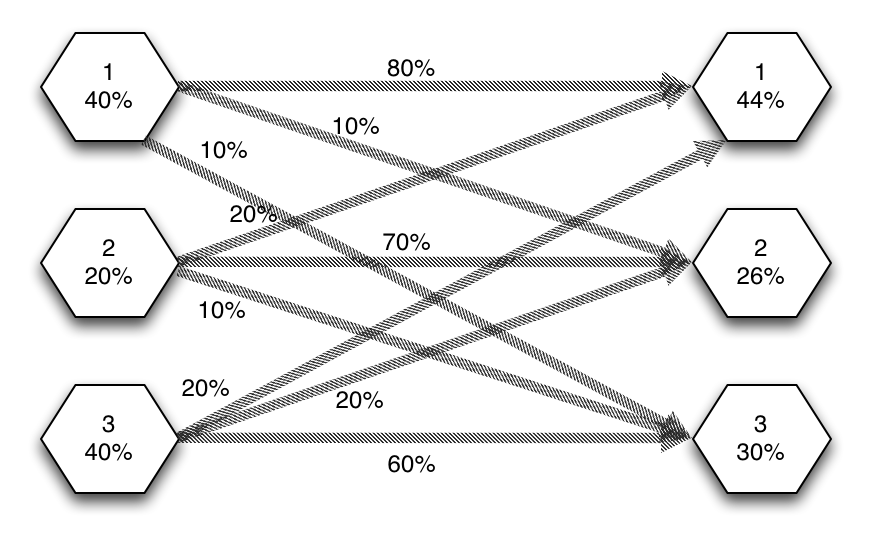
\includegraphics[width=10cm]{marktanteile_ergebnis.png}
\end{frame}

\begin{frame}{Anwendungsbeispiel - Matrizenmultiplikation}
	Bezeichnet $\pmb{K^{23}}$ die entsprechende Übergangsmatrix von Periode 2 auf Periode 3, so kann man die Übergangsmatrix von Periode 1 auf Periode 3 wie folgt berechnen:
	\[
		\pmb{K^{13}} = \pmb{K^{23}} \pmb{K^{12}}
	\]
	denn für die Marktanteile in Periode 3 gilt:
	\[
	\pmb{M^{3}}  = \pmb{K^{13}} \pmb{M^{1}} = \pmb{K^{23}} \pmb{M^{2}} = \pmb{K^{23}} \pmb{K^{12}} \pmb{M^{1}}
	\]
		Mit den Übergangsmatrizen
		\[
		\pmb{K^{12}} = \begin{pmatrix}
		0,8 & 0,2 & 0,2 \\
		0,1 & 0,7 & 0,2 \\
		0,1 & 0,1 & 0,6
		\end{pmatrix} \qquad \mbox{und} \qquad 	\pmb{K^{23}} = \begin{pmatrix}
		0,7 & 0,1 & 0,2 \\
		0,2 & 0,8 & 0,1 \\
		0,1 & 0,1 & 0,7
		\end{pmatrix}
		\]
		
\end{frame}

\begin{frame}{Anwendungsbeispiel - Matrizenmultiplikation}
		\begin{equation*}
		\begin{array}{@{}rl}
		\pmb{K^{12}} \ = \
		\left(
		\begin{array}{c} 0,8 \\ 0,1 \\ 0,1
		\end{array}
		\fbox{$\begin{array}{c} 0,2 \\  0,7 \\ 0,1 \end{array}$}
		\begin{array}{c} 0,2 \\ 0,2 \\ 0,6
		\end{array}
		\right) \, &
		\\
		\pmb{K^{23}} \ = \
		\left(
		\begin{array}{c}
		0,7 \quad 0,1 \quad 0,2 \\
		\fbox{$0,2 \quad 0,8 \quad 0,1$} \\
		0,1 \quad 0,1 \quad 0,7
		\end{array} \right) \
		\left(
		\begin{array}{c} 0,59 \\ 0,25 \\ 0,16 \end{array}
	\begin{array}{c} 0,23 \\ \fbox{0,61} \\ 0,16
		\end{array}
	\begin{array}{c} 0,28 \\ 0,26 \\ 0,46 \end{array}
		\right) &  = \ \pmb{C}
		\end{array}
		\end{equation*}
		
		Damit sind die Marktanteile im dritten Jahr:
		\[
			\pmb{M^{3}} = \pmb{K^{13}} \pmb{M^{1}} = \begin{pmatrix}
				0,59 & 0,23 & 0,28 \\
				0,25 & 0,61 & 0,26 \\
				0,16 & 0,16 & 0,46
			\end{pmatrix} \begin{pmatrix}
				40 \% \\ 20 \% \\ 40 \%
			\end{pmatrix} = \begin{pmatrix}
				39,4 \% \\ 32,6 \% \\ 28 \%
			\end{pmatrix}
		\]
		
\end{frame}

\subsubsection{Determinanten}

\begin{frame}{Determinanten - Motivation}
	Für das $2\times 2$-Gleichungssystem
	\begin{align*}
		a_{11} x_{1} + a_{12} x_{2} = b_{1} \\
		a_{21} x_{2} + a_{22} x_{2} = b_{2}
	\end{align*}
	kann man auch schreiben
	\[
	\pmb{A} \vv{x} =
	\begin{pmatrix}
		a_{11} & a_{12} \\
		a_{21} & a_{22}
	\end{pmatrix} \begin{pmatrix}
	x_{1} \\ x_{2}
	\end{pmatrix} = \begin{pmatrix}
		b_{1} \\ b_{2}
	\end{pmatrix} = \vv{b}
	\]
	oder für das Gauß-Jordan-Verfahren:
	\[
		\left(\begin{array}{cc|c}
			a_{11} & a_{21} & b_{1} \\
			a_{12} & a_{22} & b_{2}
		\end{array}\right)
	\]
\end{frame}

\begin{frame}{Determinanten - Motivation}
	Multipliziert man für das Gauß-Jordan-Verfahren
	\[
	\left(\begin{array}{cc|c}
	a_{11} & a_{21} & b_{1} \\
	a_{12} & a_{22} & b_{2}
	\end{array}\right)
	\]
	\begin{itemize}
	\item die erste Zeile mit $a_{22}$ und die zweite Zeile mit $a_{12}$ und subtrahiert die beiden Ergebnisse für die erste Zeile
	\item die zweite Zeile mit $a_{11}$ und die erste Zeile mit $a_{21}$ und subtrahiert die beiden Ergebnisse für die zweite Zeile,
	\end{itemize}
	so erhält man:
	\[
	\left(\begin{array}{cc|c}
	a_{11}a_{22} - a_{12}a_{12} & 0  & a_{22}b_{1} - a_{12}b_{2} \\
	0 & a_{11}a_{22} - a_{12}a_{12} & a_{11}b_{2} - a_{21}b_{1}
	\end{array}\right)
	\]
	Das hat schon Diagonalform und die Faktoren vor $x_{1}$ und $x_{2}$ sind gleich, nämlich die \textbf{Determinante von $\pmb{A}$}
	
	\fbox{$ \det \pmb{A} := a_{11} a_{22} - a_{12} a_{21}$}
\end{frame}

\begin{frame}{Determinante - Definition $2 \times 2$}
	\begin{definition}
		Die \textbf{Determinante} ist eine reelle Zahl, die aus den Elementen einer \emph{quadratischen Matrix} nach bestimmten Vorschriften berechnet wird.
		
		Diese Zahl ist nützlich u.a. für die Entscheidung über die Lösbarkeit von linearen Gleichungssystemen.
	\end{definition}
	\begin{definition}
		Für eine quadratische $2 \times 2$-Matrix
		\[
			\pmb{A} = 	\begin{pmatrix}
			a_{11} & a_{12} \\
			a_{21} & a_{22}
			\end{pmatrix}
		\]
		ist die Determinante
		\[
		\det \pmb{A} := \det \begin{vmatrix}
		a_{11} & a_{12} \\
		a_{21} & a_{22}
		\end{vmatrix} := a_{11} a_{22} - a_{21} a_{12}
		\]
	\end{definition}
\end{frame}

\begin{frame}{Determinante - Definition $3 \times 3$}
	\begin{definition}
		Für eine $3 \times 3$-Matrix \[
		\pmb{A} = \begin{pmatrix}
		a_{11} & a_{12} & a_{13} \\
		a_{21} & a_{22} & a_{23} \\
		a_{31} & a_{32} & a_{33}
		\end{pmatrix}
		\]
		lautet die Determinante $\det A$
		\fbox{
		{\scriptsize
		$a_{11} a_{22} a_{33} + a_{12} a_{23} a_{31} + a_{13} a_{21} a_{32} - a_{31} a_{22} a_{13} - a_{32} a_{23} a_{11} - a_{33} a_{21} a_{12} $ } }
	\end{definition}
\end{frame}

\begin{frame}{Determinanten - Regel von Sarrus für $3 \times 3$-Determinanten}
	\begin{bemerkung}
	Für $3 \times 3$-Matrizen läßt sich die Formel für die Determinante mit der Regel von Sarrus herleiten:
\begin{center}
\begin{tikzpicture}
\matrix [%
matrix of math nodes,column sep=1em,row sep=1em,ampersand replacement=\& ] (sarrus) {%
	a_{11} \& a_{12} \& a_{13} \& a_{11} \& a_{12} \\
	a_{21} \& a_{22} \& a_{23} \& a_{21} \& a_{22} \\
	a_{31} \& a_{32} \& a_{33} \& a_{31} \& a_{32} \\
};

\path ($(sarrus-1-3.north east)+(0.5em,0)$) edge[dotted] ($(sarrus-3-3.south east)+(0.5em,0)$)
(sarrus-1-1)                          edge         (sarrus-2-2)
(sarrus-2-2)                          edge         (sarrus-3-3)
(sarrus-1-2)                          edge         (sarrus-2-3)
(sarrus-2-3)                          edge         (sarrus-3-4)
(sarrus-1-3)                          edge         (sarrus-2-4)
(sarrus-2-4)                          edge         (sarrus-3-5)
(sarrus-3-1)                          edge[dashed] (sarrus-2-2)
(sarrus-2-2)                          edge[dashed] (sarrus-1-3)
(sarrus-3-2)                          edge[dashed] (sarrus-2-3)
(sarrus-2-3)                          edge[dashed] (sarrus-1-4)
(sarrus-3-3)                          edge[dashed] (sarrus-2-4)
(sarrus-2-4)                          edge[dashed] (sarrus-1-5);

\foreach \c in {1,2,3} {\node[anchor=south] at (sarrus-1-\c.north) {$+$};};
\foreach \c in {1,2,3} {\node[anchor=north] at (sarrus-3-\c.south) {$-$};};
\end{tikzpicture}
\end{center}
\end{bemerkung}
\end{frame}

\begin{frame}{Determinantenentwicklungssatz von Laplace}
	Für die Berechnung von Determinanten von Matrizen mit mehr Spalten (bzw. Zeilen) braucht man den \textbf{Entwicklungssatz von Laplace}:
	\begin{theorem}
		Die Determinante einer $(n \times n)$-Matrix $\pmb{A}$ kann mit dem Entwicklungß atz von Laplace berechnet werden:
		\[
		\det \pmb{A} = \sum\limits_{k=1}^{n} (-1)^{i+k} a_{ik} \det A_{ik} = \sum\limits_{i=1}^{n} (-1)^{i+k} a_{ik} \det A_{ik}
		\]
		wobei
		\begin{itemize}
		\item $i$ für eine beliebige Zeile bzw. $k$ für eine beliebige Spalte steht und
		\item $A_{ik}$ die Matrix bezeichnet, die entsteht, wenn man in der Matrix $\pmb{A}$ die $i$-te Zeile und die $k$-te Spalte streicht, und deren Determinante man \textbf{Unterdeterminanten} oder (zusammen mit dem Vorfaktor $(-1)^{i+k}$) \textbf{Adjunkte} nennt.
		\end{itemize}
	\end{theorem}
\end{frame}

\begin{frame}{Determinantenentwicklungssatz von Laplace}
	\begin{bemerkung}
		\begin{itemize}
			\item Für die Vorfaktoren $(-1)^{i+k}$ kann man sich am besten die Matrix wie folgt in Schachbrettform vorstellen:
			\[
				\begin{vmatrix}
				+ & - & + & - & + & \cdots \\
			    - & + & - & + & - & \cdots \\
				+ & - & + & - & + & \cdots \\
				- & + & - & + & - & \cdots \\
				\vdots & \vdots & \vdots & \vdots & \vdots & \ddots
				\end{vmatrix}
			\]
			\item Die im Entwicklungssatz vorkommenden Determinanten der Matrizen $A_{ik}$ sind Determinanten von kleineren $(n-1) \times (n-1)$-Matrizen, die man entweder wieder mit dem Entwicklungssatz, der Regel von Sarrus oder einfacher berechnen kann.
			\item Man entwickelt also entweder nach einer Zeile ($i$ bleibt, einmal gewählt, fest) oder nach einer Spalte ($k$ bleibt fest).
		\end{itemize}
	\end{bemerkung}
\end{frame}

\begin{frame}{Determinantenentwicklungssatz von Laplace}
	\begin{bemerkung}
	\begin{itemize}
		\item Idealerweise entwickelt man nach der Zeile oder Spalte, in der möglichst viele 0 vorkommen, weil so die entsprechenden Summenterme wegfallen und damit die Berechnung der entsprechenden Unterdeterminanten.
		\item Man kann vor der Berechnung die Matrix mit den Umformungen aus dem Gauß-Verfahren so verändern, dass in einer Zeile oder Spalte alle Elemente bis auf eines 0 sind bzw. möglichst viele 0 entstehen.
		\item Für eine Dreiecksmatrix (sie muss nicht diagonal sein), die also alle Einträge unterhalb oder oberhalb der Diagonalen 0 hat, muss  man nur die Einträge in der Diagonalen multiplizieren. Das gilt dann natürlich auch für Diagonalmatrizen.
		\item Wenn eine Zeile oder eine Spalte vollständig aus 0 besteht, ist die Determinanten automatisch auch 0.
	\end{itemize}
	\end{bemerkung}
\end{frame}

\begin{frame}{Determinantenentwicklungssatz - Beispiel}
	Im folgenden Beispiel entwickelt man am besten nach der dritten Zeile:
	\[
	\begin{vmatrix}
	1 & 2 & 5 & 3 \\
	2 & -1 & 6 & 7 \\
	1 & 0 & 0 & 2 \\
	-2 & -3 & 1 & 2
	\end{vmatrix} = 1 \cdot \begin{vmatrix}
	2 & 5 & 3 \\
	-1 & 6 & 7 \\
	-3 & 1 & 2
	\end{vmatrix} - 2 \cdot \begin{vmatrix}
	1 & 2 & 5 \\
	2 & -1 & 6 \\
	-2 & -3 & 1
	\end{vmatrix}
	\]
	\[
	 = 1\cdot(-34) -2\cdot(-51) = 102 - 34 = 68 \]
\end{frame}

\begin{frame}{Rechenregeln für Determinanten}
	Für Determinanten gelten einige Rechenregeln:
	\begin{itemize}
		\item Vertauscht man zwei Zeilen oder zwei Spalten einer Determinante, so ändert die Determinante ihr Vorzeichen.
		\item Multipliziert man eine $n \times n$-Matrix mit einer Zahl $\lambda$, so ist die Determinante mit der $n$-fachen Potenz von $\lambda$ zu multiplizieren:
		\[
		\det \left( \lambda \pmb{A} \right) = \lambda^{n} \det \pmb{A}
		\]
		\item Die Addition oder Subtraktion des Vielfachen einer Zeile oder Spalte zu einer anderen Zeile oder Spalte ändert den Wert der Determinanten nicht.
		\item Das Transponieren einer Matrix ändert die Determinante nicht, d.h.
		\[
		\det \pmb{A} = \det \pmb{A^{T}}
		\]
		\item Die Determinate eines Matrizenproduktes ist der Produkt der Determinante der Multiplikatoren:
		\[
		\det \left(\pmb{A} \pmb{B}\right) = \det \pmb{A} \det \pmb{B}
		\]
	\end{itemize}
\end{frame}

\begin{frame}{Determinanten und Lösbarkeit von LGS}
	\begin{definition}
		Eine $n \times n$-Matrix $\pmb{A}$ heißt \textbf{regulär} oder \textbf{invertierbar}, wenn für ihre Determinante
		\[
		\det \pmb{A} \neq 0
		\]
		gilt.
		Eine Matrix $\pmb{A}$, deren Determinante $\det \pmb{A} = 0$ ist, heißt \textbf{singulär}.
	\end{definition}
	Für die Lösbarkeit eines linearen Gleichungssystems $\pmb{A}\vv{x} = \vv{b}$ gibt es vier mögliche Fälle:
	\small{
	\begin{tabular}{|c|c|c|}
		\hline
		& homogen $\vv{b}=0$ & inhomogen $\vv{b} \neq 0$ \\
		\hline
		$\det \pmb{A} = 0$ & unendlich viele Lösungen & unendlich viele oder keine Lösung \\
		\hline
		$\det \pmb{A} \neq 0$ & genau eine Lösung $\vv{x}=0$ & genau eine Lösung $\vv{x} \neq 0$\\
		\hline
	\end{tabular}}
\end{frame}

\begin{frame}{Lösung linearer Gleichungssysteme - Cramersche Regel}
	\begin{theorem}
	Für die Lösung $\vv{x}$ eines (quadratischen) linearen Gleichungssystems $\pmb{A} \vv{x} = \vv{b}$ mit regulärer Koeffizientenmatrix $\pmb{A}$ gilt:
	\[
	x_{i} = \frac{\det \pmb{A_{i}}}{\det \pmb{A}}
	\]
	wobei die Matrizen $\pmb{A_{i}}$ aus $\pmb{A}$ hervorgehen, indem man die $i$-te Spalte der Matrix $\pmb{A}$ durch den Vektor $\vv{b}$ ersetzt.
 	\end{theorem}
\end{frame}

\begin{frame}{Cramersche Regel - Beispiel}
	Für das lineare Gleichungssystem
	
		\begin{align*}
		- x_{1}  + x_{2}  + x_{3} & =  0 \\
		x_{1}  -3 x_{2}  -2 x_{3} & =  5 \\
		5 x_{1}  +x_{2}  +4 x_{3} & =  3
		\end{align*}

	oder in Matrixschreibweise
	\[
	\begin{pmatrix}
	-1 & 1 & 1 \\
	1 & -3 & -2 \\
	5 & 1 & 4
	\end{pmatrix} \cdot \begin{pmatrix}x_{1} \\ x_{2} \\ x_{3} \end{pmatrix} = \begin{pmatrix}
	0 \\ 5 \\ 3
	\end{pmatrix}
	\]
	ist
	\[
	\pmb{A}= \begin{pmatrix}
	-1 & 1 & 1 \\
	1 & -3 & -2 \\
	5 & 1 & 4
	\end{pmatrix}
	\qquad
	\vv{b} = \begin{pmatrix}
	0 \\ 5 \\ 3
	\end{pmatrix}
	\]
\end{frame}

\begin{frame}{Cramersche Regel - Beispiel}
		\[
		\pmb{A}= \begin{pmatrix}
		-1 & 1 & 1 \\
		1 & -3 & -2 \\
		5 & 1 & 4
		\end{pmatrix}
		\qquad
		\vv{b} = \begin{pmatrix}
		0 \\ 5 \\ 3
		\end{pmatrix}
		\]
		und daher \footnotesize{
		\[
		\pmb{A_1}= \begin{pmatrix}
		0 & 1 & 1 \\
		5 & -3 & -2 \\
		3 & 1 & 4
		\end{pmatrix}
		\qquad
		\pmb{A_2}= \begin{pmatrix}
		-1 & 0 & 1 \\
		1 & 5 & -2 \\
		5 & 3 & 4
		\end{pmatrix}
		\qquad
		\pmb{A_3}= \begin{pmatrix}
		-1 & 1 & 0 \\
		1 & -3 & 5 \\
		5 & 1 & 3
		\end{pmatrix}
		\]
		}
		und mit der Regel von Sarrus
		\[
		\det \pmb{A_1} = -12 \qquad \det \pmb{A_2} = -48
 \qquad \det \pmb{A_3} = 36 \qquad \det \pmb{A} = 12		
 \]
	und daher
	\[
	x_{1} = \frac{-12}{12} = -1 \qquad x_{2} = \frac{-48}{12} = -4 \qquad x_{3} = \frac{36}{12} = 3
	\]	
\end{frame}
